%%%%%%%%%%%%%%%%%%%%%%%%%%%%%%%%%%%%%%%%%%%%%%%%%%%%%%%%%%%%%%%%%%%%%%%%%%%%%%%%%%%%%%
% TEMPLATE FOR PHYS250 WORKSHEET
% This template uses the Memoir class. It is a very powerful class for 
% creating documents such
% as reports, papers and theses. You can find more information at CTAN, the Comprehensive
% TeX Archive Network. These is a long manual that describes how to use Memoir.
% https://www.ctan.org/pkg/memoir?lang=en

%%%%%%%%%%%%%%%%%%%%%%%%%%%%%%%%%%%%%%%%%%%%%%%%%%%%%%%%%%%%%%%%%%%%%%%%%%%%%%%%%%%%%

\title{Matériaux pour l'Ingénieur\vspace{0.5em}\\TP n°4\vspace{0.5em}\\Compte-rendu}
\author{Jia \textsc{Fu}, Paul \textsc{Meddeb}, Louis-Justin \textsc{Tallot}}
\date{Mardi 15 juin 2021}


\documentclass[12pt,oneside,oldfontcommands]{memoir}



%	MARGIN AND HEADER/FOOTER SIZES

\setlrmarginsandblock{2.5cm}{2.5cm}{*}  		% left/right margins
\setulmarginsandblock{2.5cm}{2.5cm}{*} 			% top/bottom margins
\checkandfixthelayout							% checks the layout is correct
\setlength{\parindent}{0in}  					% no indent on start of paragraph
							


%  PACKAGES

\usepackage{amsmath,amsthm,amssymb,amsfonts}			% math fonts
\usepackage[french]{babel}								% hyphenation rules for english
\usepackage[T1]{fontenc} 
\usepackage{graphicx}
% for importing pdf files 
\usepackage{siunitx}									% si units - extremely useful
% defines the dvips color names
\usepackage[usenames,dvipsnames,svgnames,table]{xcolor}	
\usepackage{color,soul} 	% for highlight hi - hyphenation, underlining
\setulcolor{red} 										% set underline color
\setstcolor{green} 										% set overstriking color
\sethlcolor{green} 										% set highlighting color

\usepackage{fancyhdr}
\pagestyle{fancy}
\fancyhf{}
\rhead{École des Mines de Paris}
\lhead{MPI - TP n°4 - Compte-rendu}
\rfoot{\vspace{-0.7 cm}\thepage}
\lfoot{
\includegraphics[width = 3 cm]{logo_mines.png}}

%  GRAPHICS PATH

\graphicspath{{images/}{./}{images_optique/}{images_meb/}}		% put your figures in a folder called images



%  SOME NEW FUNCTIONS FOR IMPORTING FIGURES

\newcommand{\placefigure}[1]{\centerline{\includegraphics[width=2 in]{#1}}} 
\newcommand{\placefigureandscale}[2]{\centerline{\includegraphics[width=#2 in]{#1}}} 



%-------------------------------------------------------------------------------------
%	TITLE PAGE MACRO
%------------------------------------------------------------------------------------
\makeatletter
\def\maketitle{%
  \null
  \thispagestyle{empty}
  \begin{center}\leavevmode
       \vskip 2cm
       \normalfont
       
\includegraphics[width=0.5\columnwidth]{logo_mines.png}
       \vskip 1cm
    %   \textsc{\Large PHYS250 Worksheet}\\[0.5 cm]
	     {\large Mardi 15 juin 2021\par}
       \vskip 1.0cm
	\rule{\linewidth}{0.2 mm} \\[0.4 cm]
	{ \huge \bfseries \@title}\\
	\rule{\linewidth}{0.2 mm} \\[1.5 cm]
	
	\vspace{1cm}
	
	\Large{\emph{Étudiants} : Jia \textsc{Fu}, Paul \textsc{Meddeb}, Louis-Justin \textsc{Tallot}}
	\vspace{0.5cm}
	\Large{\emph{Encadrants} : Robin \textsc{Mallick}, Mohamed \textsc{Shokeir}}
	
% 	\begin{minipage}{0.5\textwidth}
% 		\begin{flushleft} \large
% 			\emph{Name:} \studentone\\
% 			Student Number: \studentonenumber
% 			\end{flushleft}
% 			\end{minipage}~
% 			\begin{minipage}{0.4\textwidth}
% 			\begin{flushleft} \large
% 			\emph{Partner:} \studenttwo\\
% 			Student Number: \studenttwonumber
% 		\end{flushleft}
% 	\end{minipage}\\[2 cm]
   \end{center}
   \vfill
   \null
   \cleardoublepage
  }
\makeatother


%	START OF DOCUMENT


\begin{document}
%\large 
\maketitle
\frontmatter
\let\cleardoublepage\clearpage
\mainmatter
\sloppy




\section*{Introduction générale}
% texte pour l'introduction générale

Les réacteurs d'avion sont des assemblages complexes de pièces soumises à de
très fortes contraintes. En effet, l'air qui est aspiré à la température 
ambiante, est ensuite compressé dans plusieurs étages de compresseurs, 
avant de rencontrer le kérosène dans la chambre de combustion. Les températures
atteignent alors les \SI{1250}{\celsius}, et l'air est ensuite éjecté du réacteur
et propulse l'avion.


\begin{figure}[H]
    \centering
    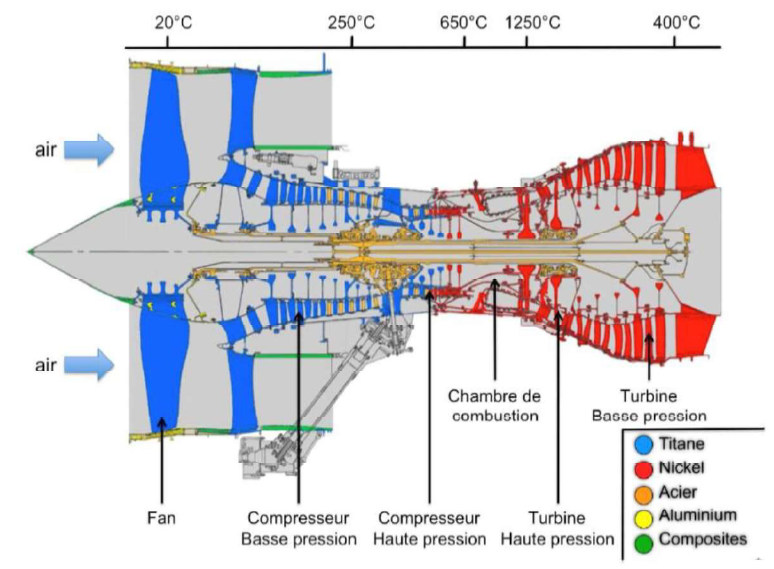
\includegraphics[width=0.55\textwidth]{images/coupe_CFM56.png}
    \caption{Vue en coupe d'un moteur type CFM56}
    \label{fig:CFM56}
\end{figure}


Les aubes de la turbine haute pression sont ainsi soumises à des conditions très rudes :
elle tournent en continu pendant plusieurs heures à $10000$ tours par minute sous une 
température de 1250°C. C'est pourquoi plusieurs industriels dont Safran cherchent à développer
des aubes de turbine résistantes au fluage, notamment grâce à un traitement thermique. 
Cela permet d'augmenter la température dans le compresseur et donc l'efficacité du moteur, 
ainsi que la durée de vie de celui-ci.




\section*{Introduction scientifique}
L'aube de turbine évolue dans un environnement particulièrement oxydant et corrosif. 
En particulier la haute température (\SI{1250}{\celsius}) et les contraintes auxquelles est soumise 
l'aube sont propices au fluage, c'est à dire la déformation lente de la pièce soumise à une contrainte constante sous une forte température. Il convient donc d'étudier l'influence des 
caractéristiques micro-structurales sur le fluage, dont la diffusion est le principal 
vecteur puisque c'est sous son effet que les atomes migrent en provoquant l'allongement du matériau.\\


La première forte évolution technologique dans le domaine a été le passage à la conception 
d'aube mono-cristallines vers la fin des années 1970. En effet les joints de grain sont des
"autoroutes à diffusion" et le fait de n'avoir qu'un seul grain améliore grandement les 
performances en fluage. Ainsi, les aubes sont aujourd'hui réalisées en super-alliage de 
nickel à base d'aluminium par refroidissement et croissance d'un unique grain initial.\\


D'autre part, les défauts micro-structurels ont également un impact sur la résistance 
mécanique du matériau. Par exemple, la trop forte présence de pores pose problème, 
ainsi que les hétérogénéités chimiques. Lors de l'étape de fonderie, le refroidissement
n'est pas homogène et certaines zones se solidifient avant d'autres ce qui fait 
que le liquide est appauvri de certains éléments : on parle alors de dendrites. 
C'est ce contraste chimique résultant entre dendrites et zones inter-dendritiques
qui diminue les capacités de résistance mécanique de la structure.\\


À l'échelle des phases, un agencement ordonnée des phases $\gamma'$ dans la 
matrice $\gamma$ permet de moins laisser se propager les champs de contraintes de 
certains défauts tel que la dislocation.\\


Deux questions se posent : Quelles sont les caractéristiques micro-structurelles 
optimales du point de vue de la résistance du matériau au fluage et aux autres 
contraintes de son milieu ? Et dans quelle mesure différents traitements thermiques 
permettent-ils d'atteindre cet optimum ?\\


La première question est traitée par les industriels qui ont déterminé différentes 
caractéristiques reconnues comme optimales (fraction volumique de phase $\gamma'$, 
taille des précipités de phase $\gamma'$, différence des paramètres de maille 
entre $\gamma$ et $\gamma'$...).\\


Nous nous concentrons donc dans ce TP sur l'influence du traitement thermique en observant l'organisation et les défauts de la micro-structure après chaque étape de ce traitement.



\section*{Objectifs}
Pour pouvoir obtenir la microstructure composée des phases $\gamma$ et $\gamma'$
avec des taille et fraction de précipités optimales, les superalliages à base de
Nickel sont soumis à une gamme de traitements thermiques : remise en solution puis
trempe, premier revenu et deuxième revenu. L’objectif de la remise en solution
(à des températures correspondantes au domaine monophasé $\gamma$) est de faire
disparaître les défauts qui sont apparus pendant le procédé de fonderie : 
ségrégations chimiques et zones d’agrégats eutectiques ($\gamma / \gamma'$).

Pendant la trempe (pour revenir à une température correspondant au domaine
$\gamma + \gamma'$), la microstructure issue de la remise en solution est figée 
et il n’y aurait pas de transformation de phase. Les premier et deuxième revenus 
(à des températures correspondantes au domaine biphasé $\gamma / \gamma'$) conduisent
à la précipitation et croissance de la phase $\gamma'$ dans la matrice $\gamma$. 
Les propriétés finales des superalliages à base de Nickel dépendent de la microstructure 
finale en termes de taille et de fraction de précipités $\gamma'$ ainsi que de la 
fraction de défauts issues du procédé de fonderie qui n’ont pas disparu pendant 
les traitements thermiques.


L’objectif de ce travail pratique est d’étudier l’influence des traitements thermiques 
sur la microstructure et sur les défauts formés pendant le procédé de fonderie : pores, 
zones d’agrégats eutectiques et hétérogénéités chimiques entre dendrites et zones 
inter-dendritiques. Pour cela, des observations de microstructures couplées avec de 
l’analyse d’image seront réalisées.


\section*{Démarche mise en œuvre}

\begin{enumerate}
    \item Préparation métallographique des échantillons : polissage.
    \item Observations des microstructures au microscope optique.
    \item Attaque chimique à l’eau régale.
    \item Observation des microstructures au microscope électronique à balayage (MEB)
    \item Analyses d’images : à partir des images obtenues au microscope optique (au moins 5 champs d’observation par échantillon), déterminer les fractions de défauts observés (agrégats
    eutectiques ($\gamma / \gamma'$), pores et autres).
    \item Etude de la ségrégation chimique des éléments en fonction du traitement thermique par
    profils de composition chimique par analyse dispersive en énergie (EDS).
    \item Analyse des résultats :
        \begin{enumerate}[label=\alph*]
            \item Conclusion sur les types de défauts observés à l’état brut de fonderie. Donner une explication quant à l’apparition de ces défauts.
            \item Tracer les courbes d’évolution des fractions de défauts en fonction des traitements thermiques reçus.
            \item Conclure quant à l’influence des traitements thermiques sur la fraction de défauts et sur la microstructure $\gamma / \gamma'$. 
        \end{enumerate}
\end{enumerate}



\section*{Description des outils utilisés}

\begin{figure}[H]
    \centering
    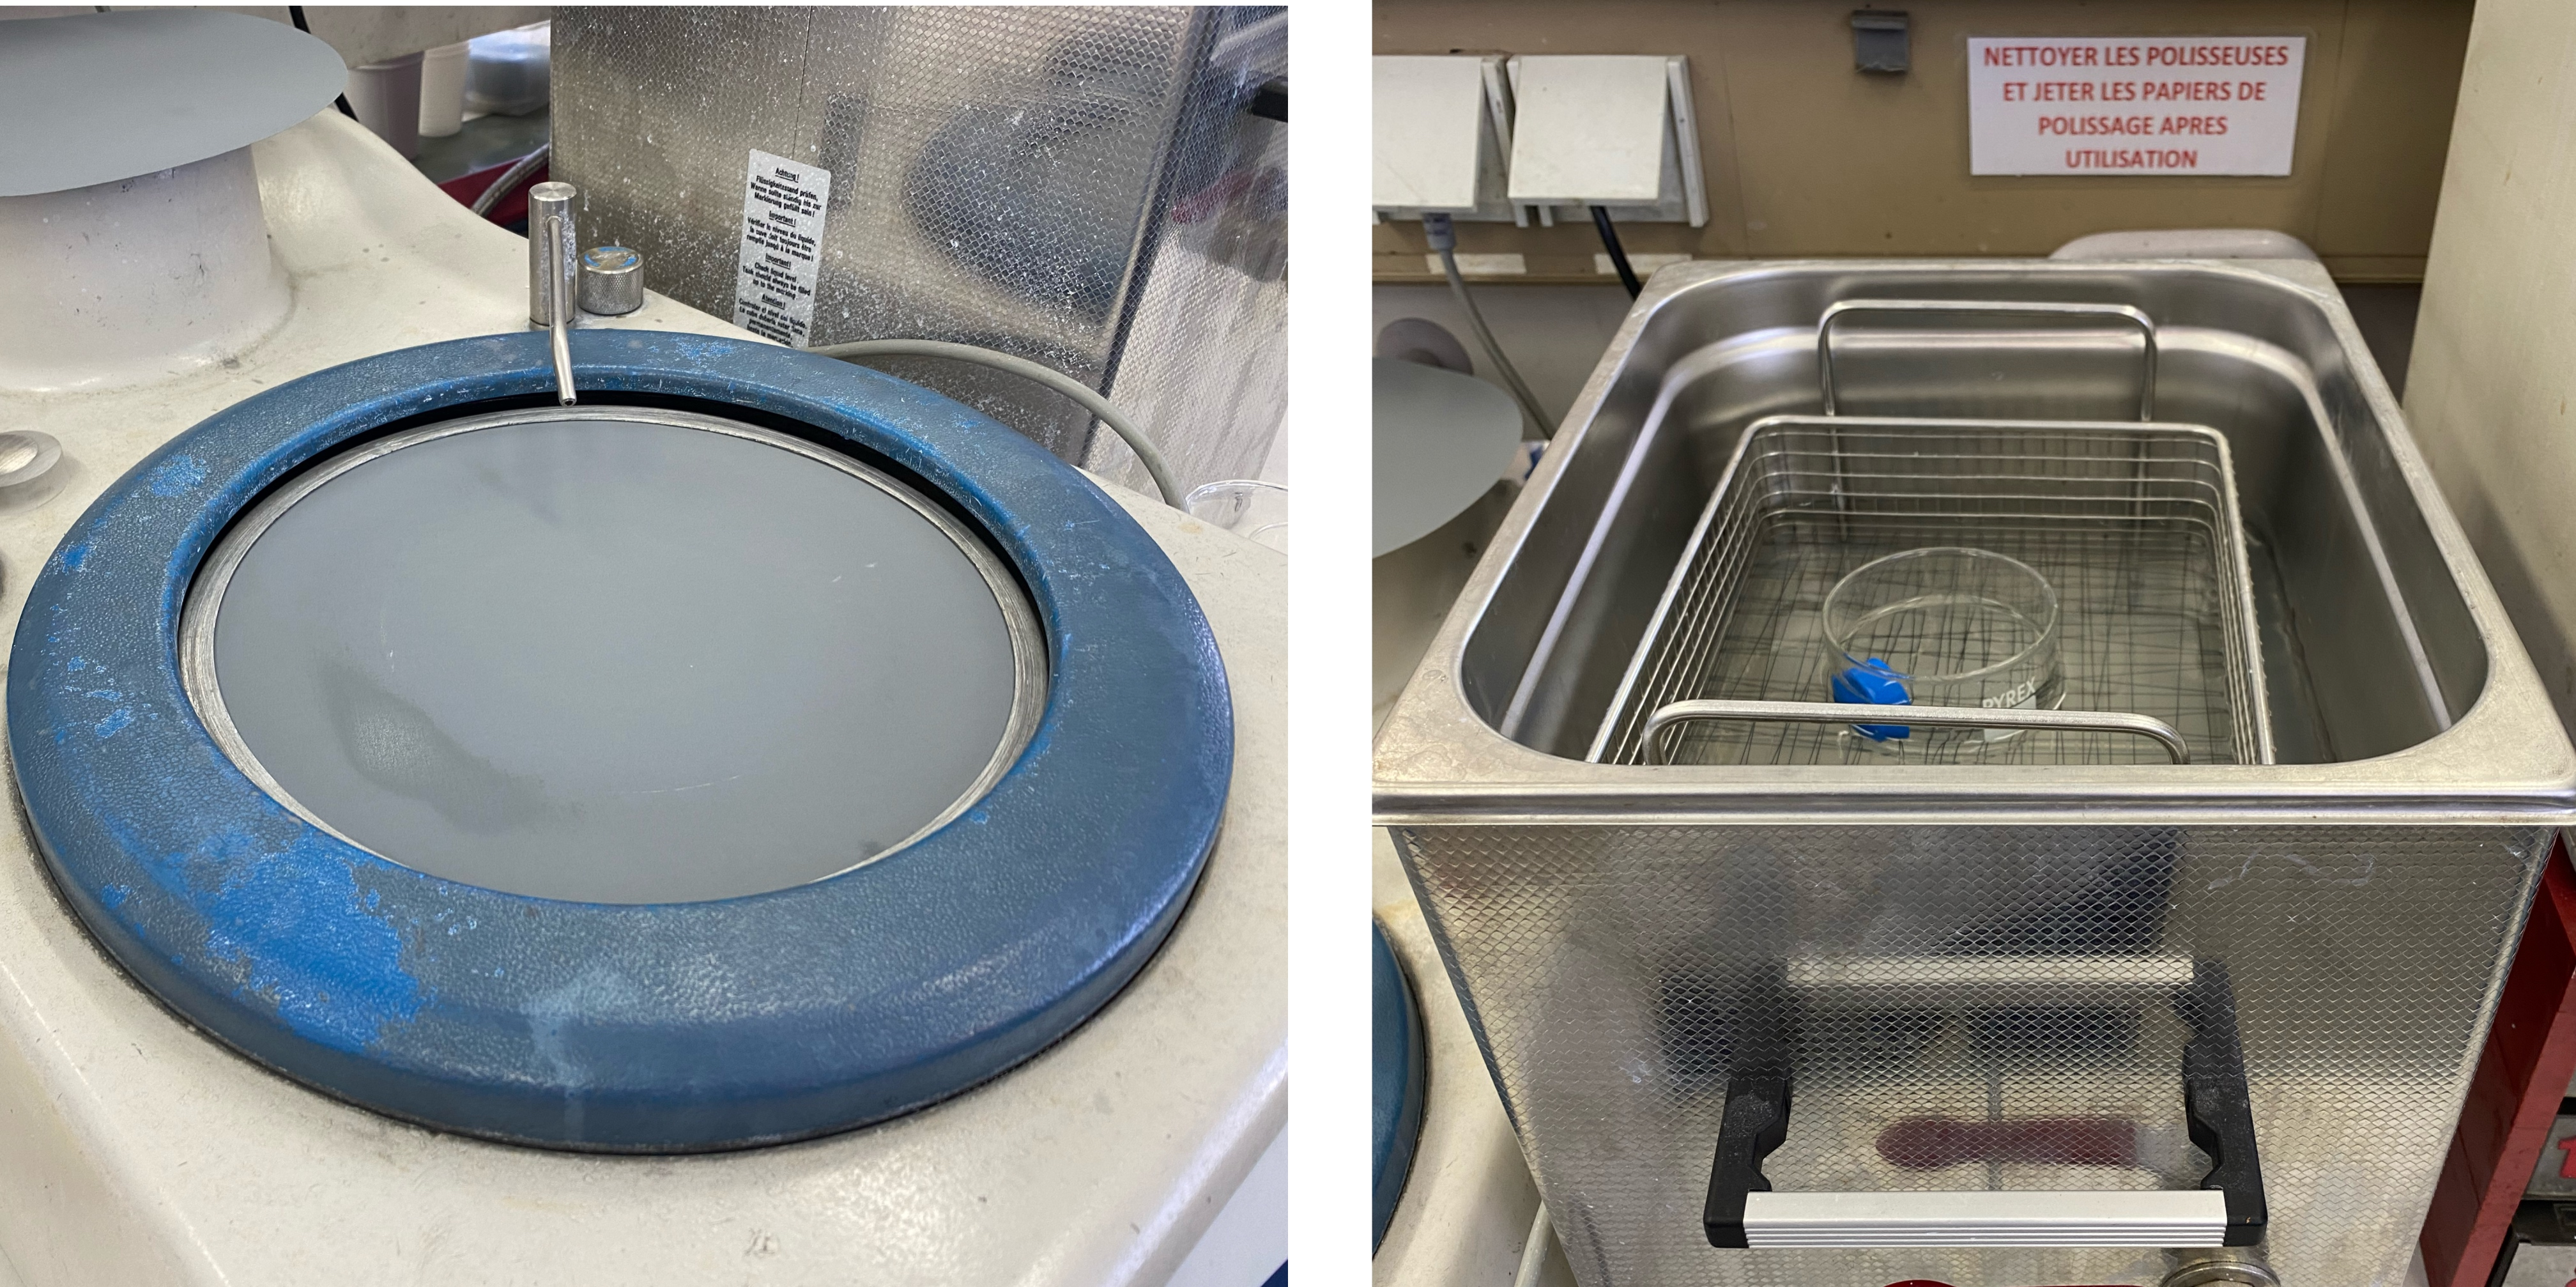
\includegraphics[width=0.55\textwidth]{images/WechatIMG1126.jpeg}
    \caption{Polisseur tournant et bain à ultrasons}
    \label{fig:polisseur_bain_ultrasons}
\end{figure}

\\\\
L'étape de polissage et nettoyage est cruciale pour ne pas avoir 
trop de défauts à la surface de l'échantillon:
on polit la pièce sur un polisseur tournant (1200 -> 2400 (eau)), puis on la passe au bain à ultrasons 2 minutes pour la nettoyer.
Ensuite on fait le passage à 2µm et 1µm (lubrifiant),
puis on la repasse au bain à ultrasons.\\
\\
\\

\begin{figure}[H]
    \centering
    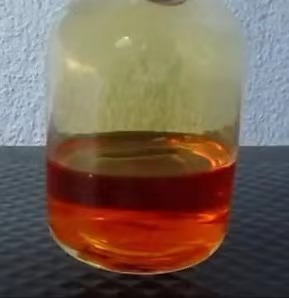
\includegraphics[width=0.35\textwidth]{images/WechatIMG1128.jpeg}
    \caption{La solution d'eau régale prête à l'emploi}
    \label{<label>}
\end{figure}
\\
On utilise un mélange composé de deux tiers d'acide chlorhydrique 
et d'un tiers d'acide nitrique.
On attend 2 minutes que les deux acides réagissent ensemble.
On observe que la solution passe de transparente à jaune-orangée.
Puis on fait tremper les pièces 45 secondes chacune dans la solution.
\\


\begin{figure}[H]
    \centering
    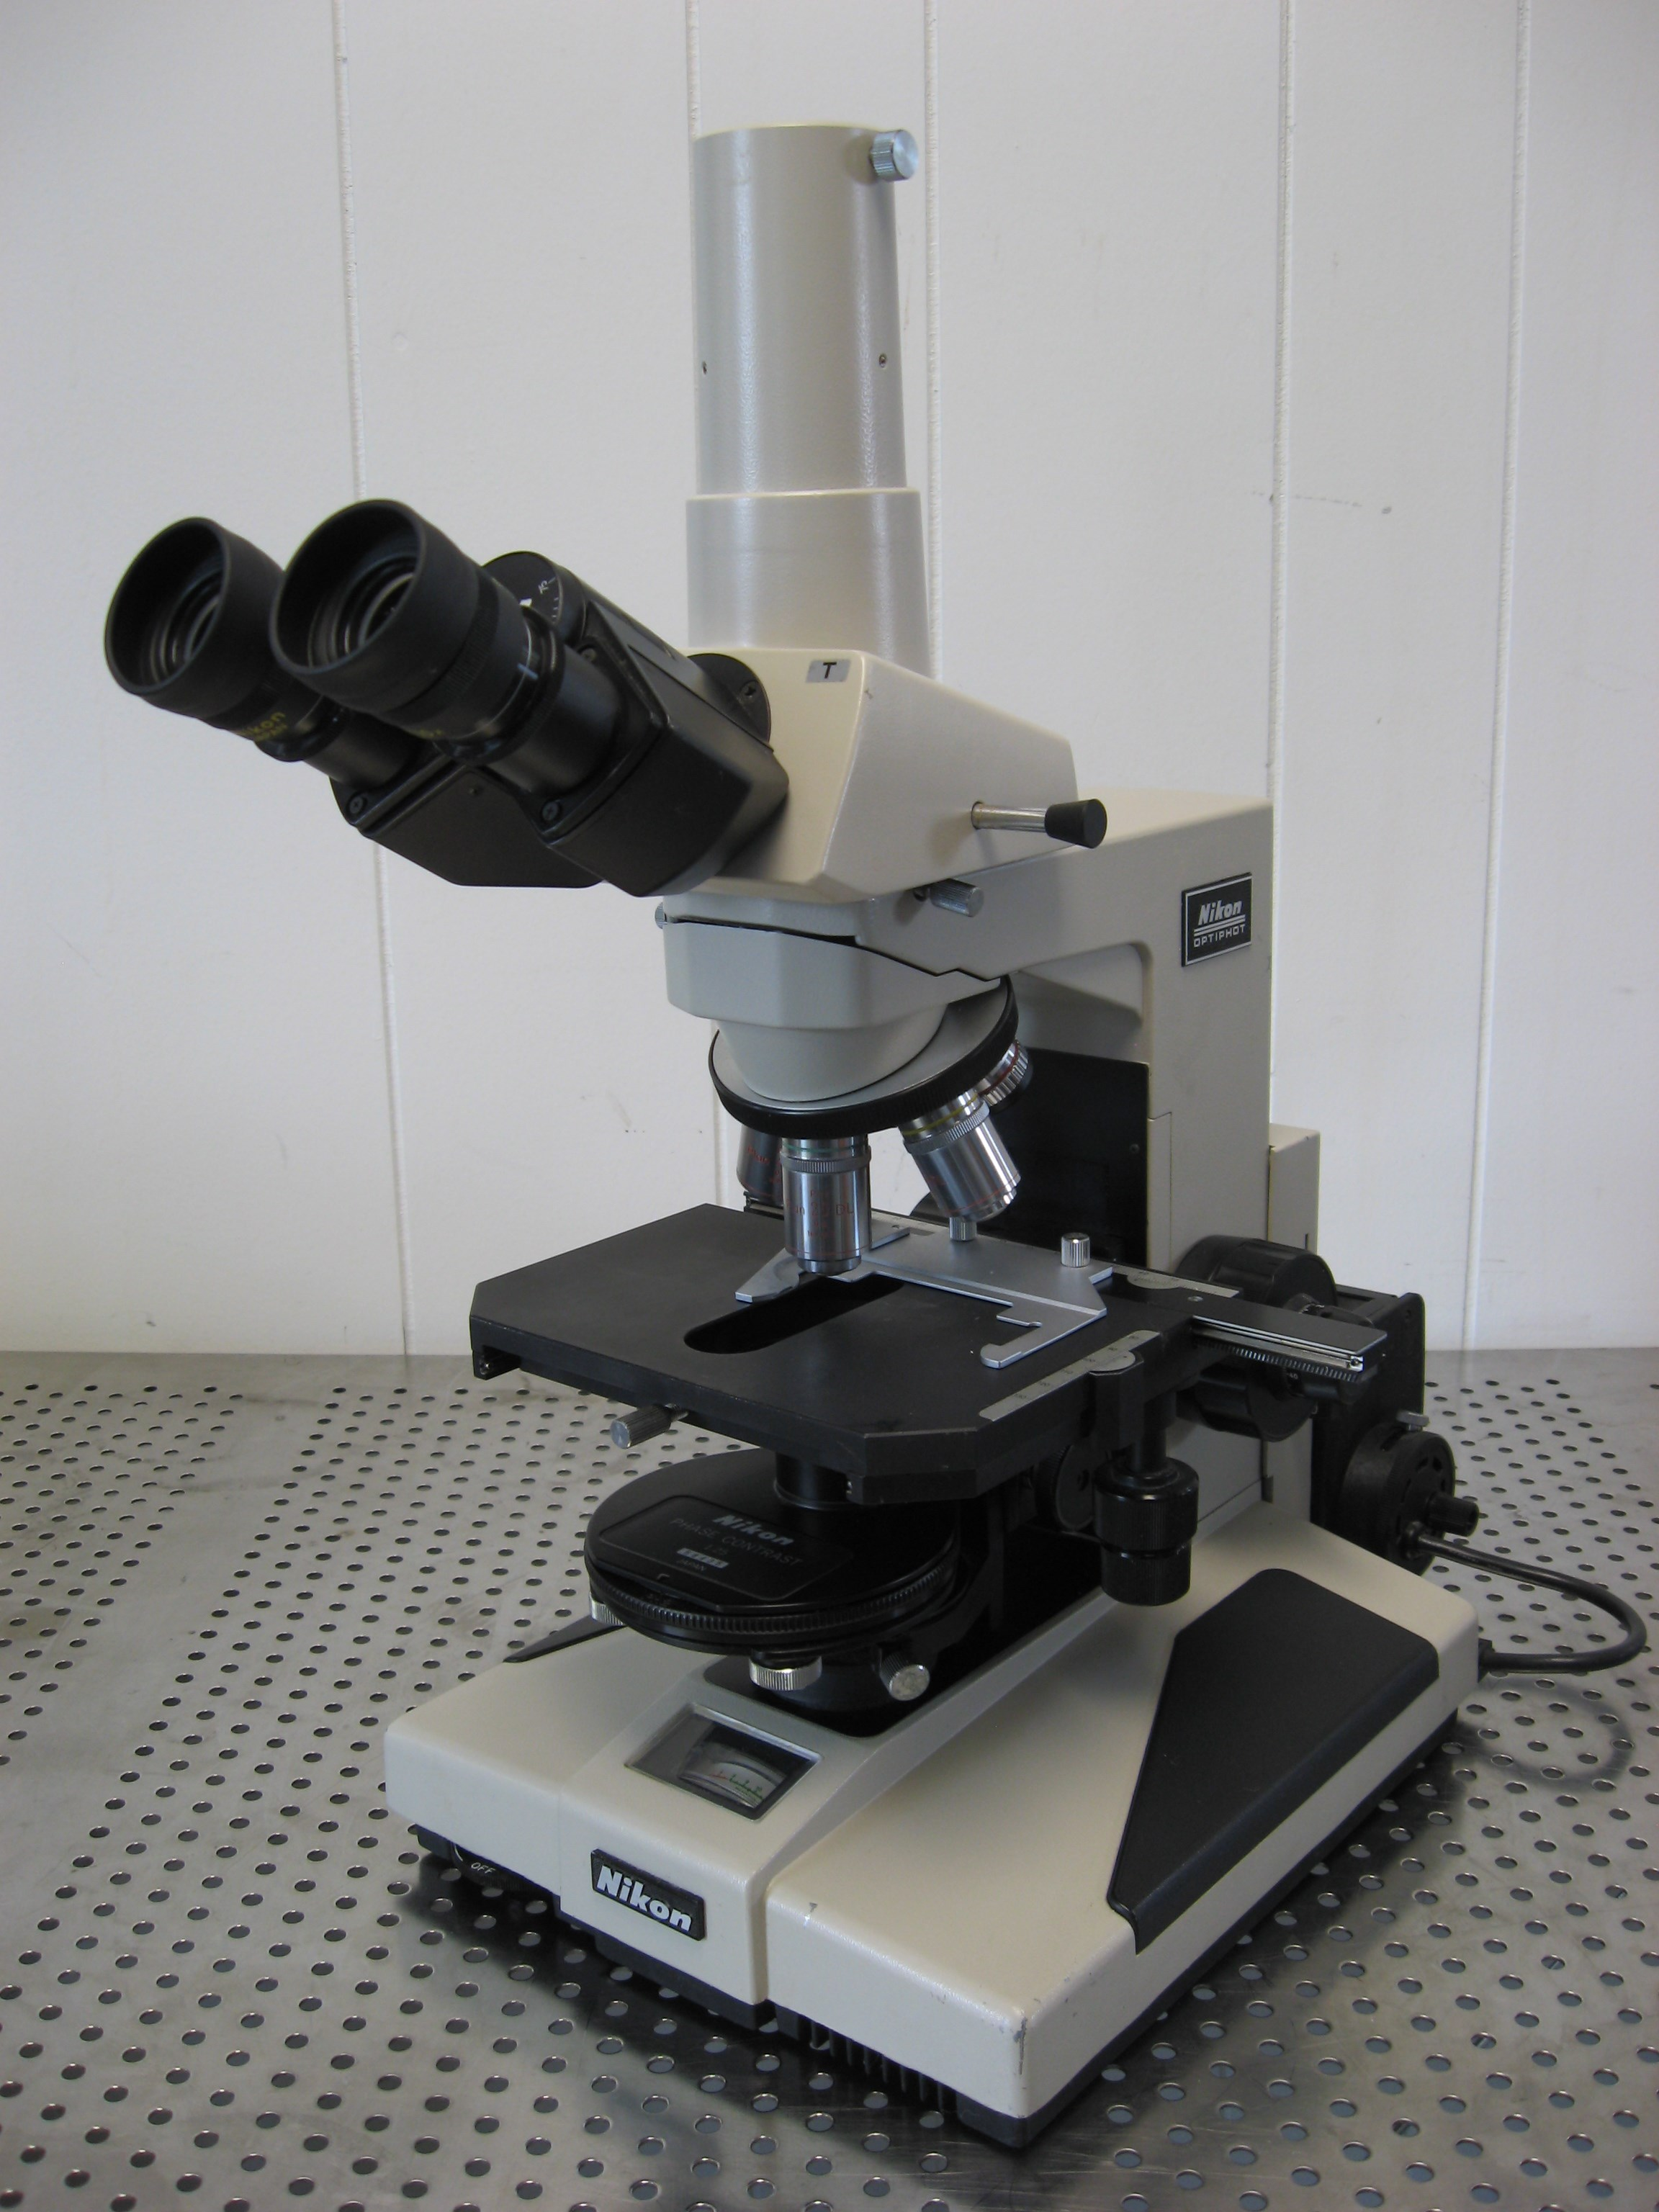
\includegraphics[width=0.35\textwidth]{images/optique.jpg}
    \caption{Le microscope optique utilisé pour examiner la surface des échantillons}
    \label{<label>}
\end{figure}
\\
Le microscope optique permet d'observer nos échantillons à l'échelle de la centaine de $\mu m$ ce qui permet de rapidement repérer les défauts les plus gros tels que les pores ou les fissures.
\\


\begin{figure}[H]
    \centering
    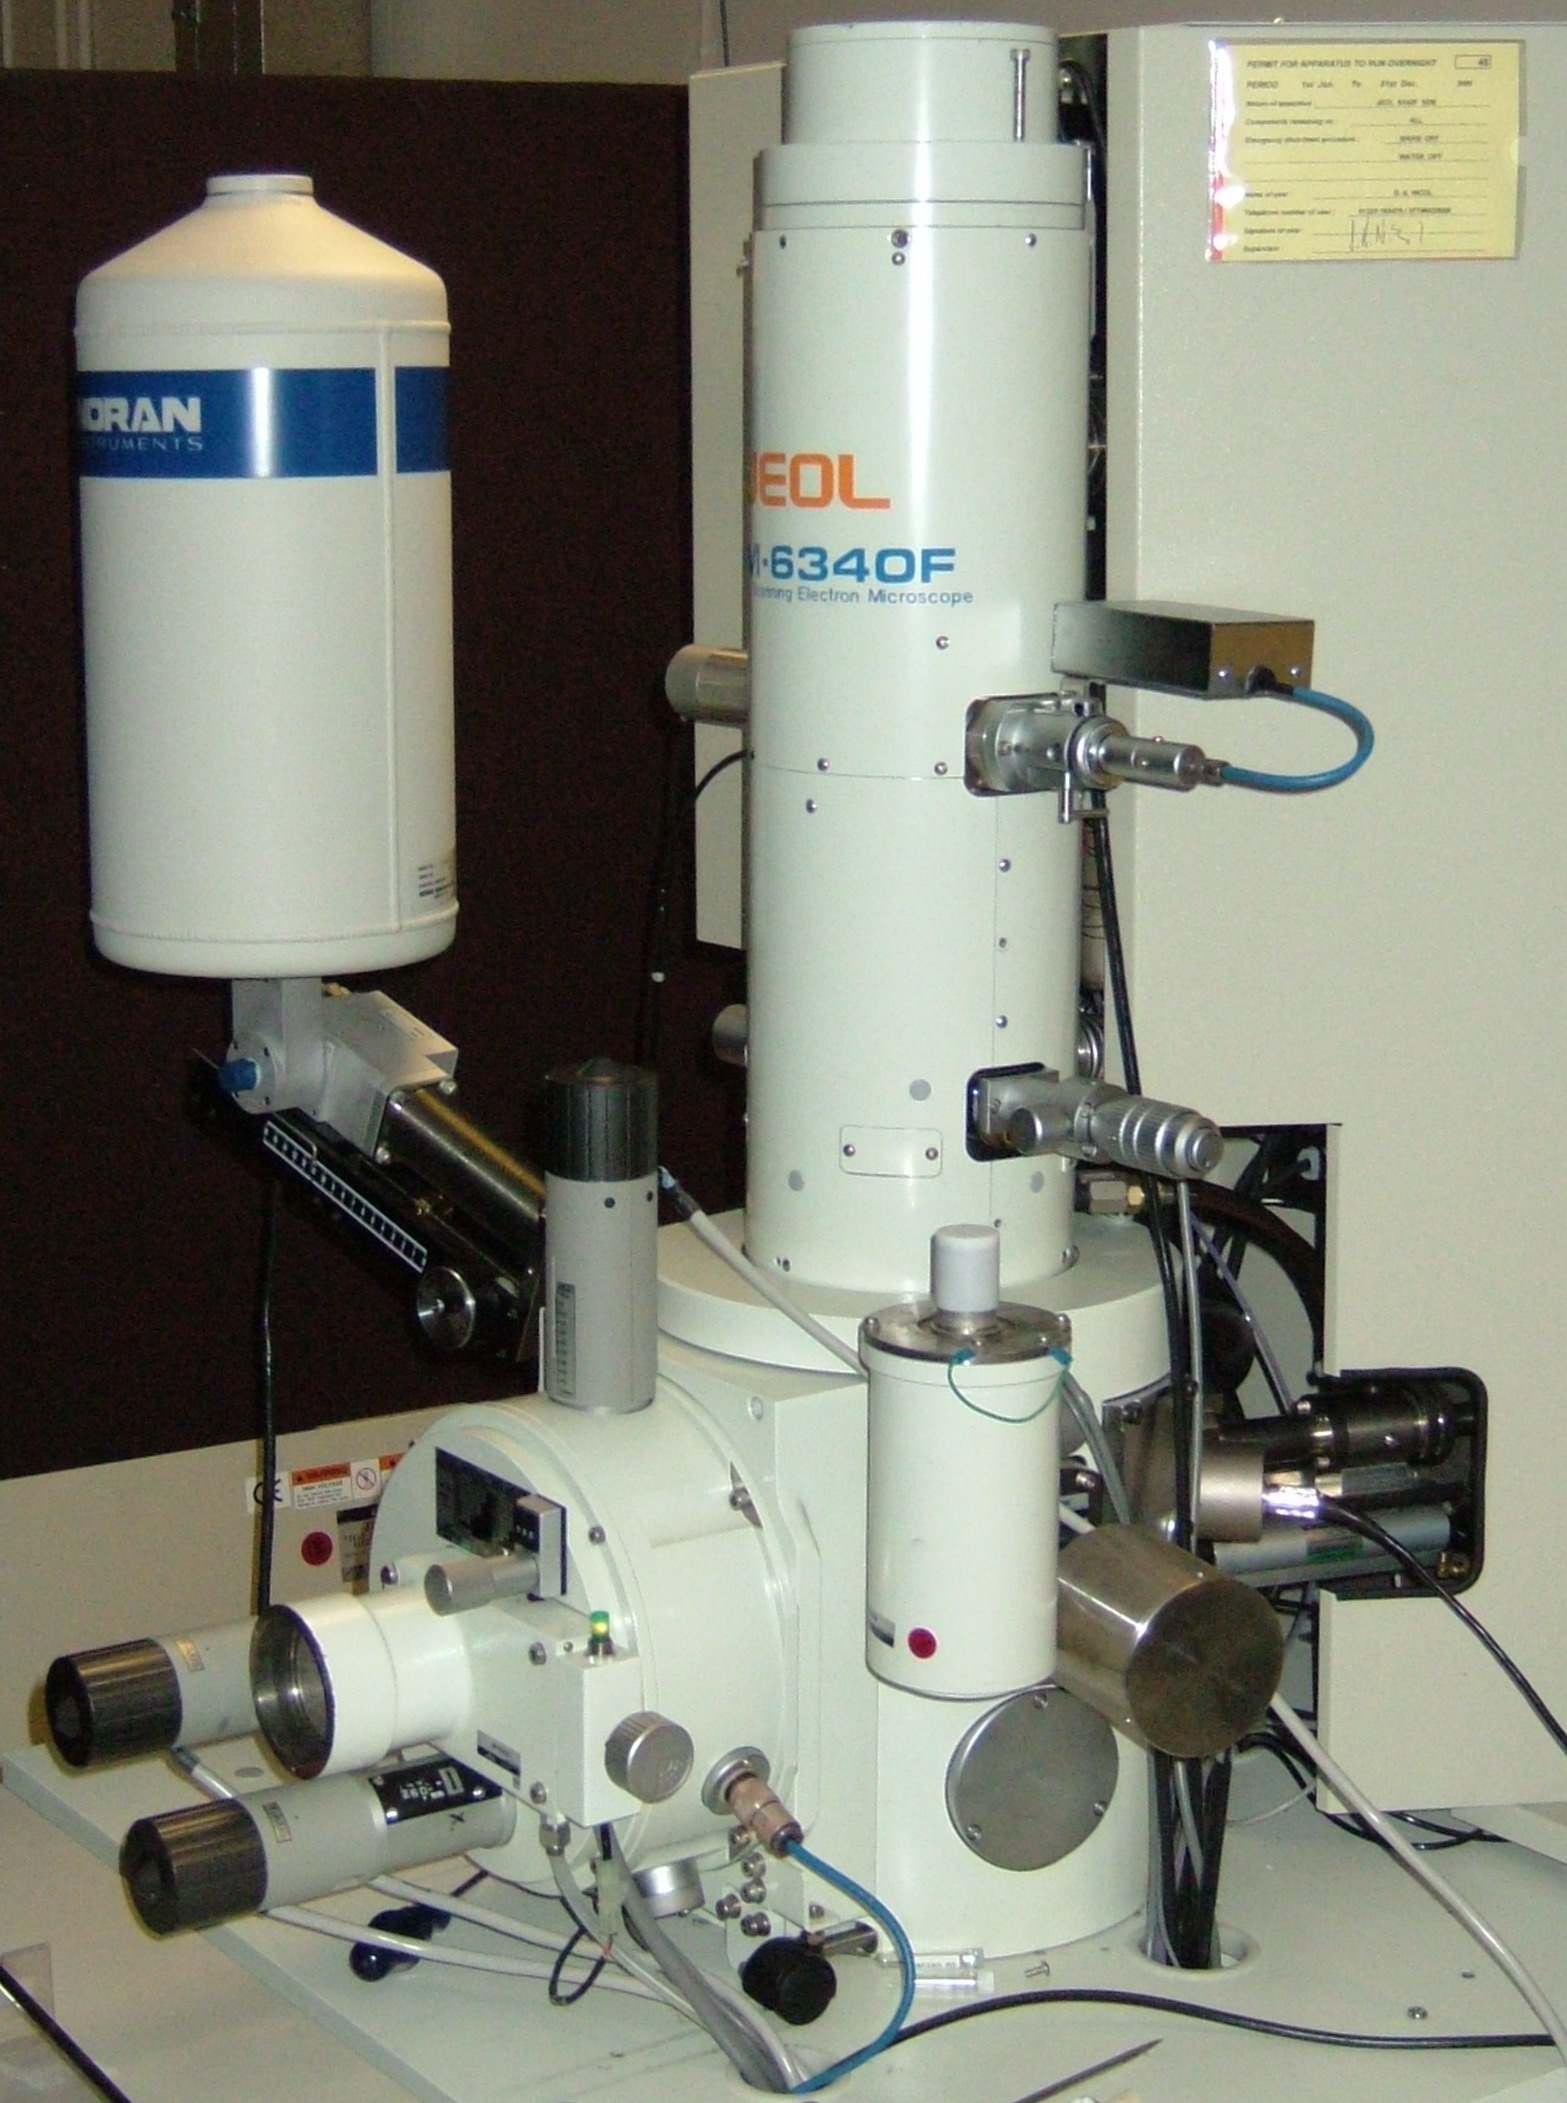
\includegraphics[width=0.4\textwidth]{images/JEOL_JSM-6340F.jpg}
    \caption{Microscope électronique à balayage pour observer la microstructure des échantillons}
    \label{<label>}
\end{figure}
\\
Des observations au MEB (microscope électronique à balayage) sont réalisées après refroidissement sous haute contrainte. Le microscope optique ne nous permettait pas d'observer l'influence du traitement thermique sur l'agencement des phases $\gamma$ et de $\gamma'$. La résolution du MEB de l'ordre du $\mu m$ nous permet d'observer la phase $\gamma'$ dans la matrice $\gamma$ ainsi que les éventuels agrégats eutectiques. La détection d'électrons rétro-diffusés permet de plus de voir à l'image les phases $\gamma$ et $\gamma'$. En effet les atomes légers de la phase $\gamma'$ sont moins déviés que les atomes plus lourds de la phase $\gamma$. Ainsi les couloirs de matrice $\gamma$ apparaissent en blanc et la phase $\gamma'$ apparaît en noir.
\newpage



\section*{Présentation des résultats obtenus}
Nous avons ainsi étudié trois types d'échantillons différents :\\
\begin{itemize}
    \item Le brut, monocristallin, en sortie de fonderie
    \item L'alliage après remise en solution (premier traitement thermique)
    \item L'alliage en fin de traitement, après les deux revenus.\\
\end{itemize}


Nous devons donc étudier leur microstructure pour déterminer l'influence des 
différents traitements thermiques sur l'alliage, étant donné que cette microstructure
est le paramètre clé qui va déterminer les propriétés mécaniques de l'alliage,
et notamment sa résistance au fluage.

\subsection*{Echantillon brut de fonderie}

Étudions tout d'abord les propriétés du brut sortant de la fonderie.\\


\begin{figure}[H]
    \centering
    
\includegraphics[width=0.75\textwidth]{images_optique/brut2.pdf}
    \caption{Echantillon brut de fonderie vu au microscope optique}
    \label{fig:brut_optique}
\end{figure}


Vu au microscope optique, sa surface (après polissage) est lisse
et présente peu de défauts. Cependant, la surface possède 
également de petites tâches noires : ces tâches sont des \emph{pores},
c'est à dire des trous à la surface de l'échantillon. Il y a à ces endroits 
des lacunes importantes dans la maille cristalline, et il manque donc 
une petite portion du matériau. Nous observons également de plus 
petites tâches grises : il s'agit d'agrégats eutectiques, formés 
lors du refroidissement du liquide.\\



On mesure la proportion de défauts visibles au microscope optique à l'aide du 
logiciel d'analyse d'images ImageJ. Nous obtenons les résultats suivants : \\


\begin{table}[H]
    \centering
    \caption{Proportion des différents défauts dans l'échantillon brut de fonderie}
    \begin{tabular}{|c|c|}
        \hline
        \textbf{Type de défaut}  & \textbf{Proportion observée}  \\
        \hline
        Pores               & $0,340$ \% \\
        Agrégats eutectiques & $0,252$ \% \\
        \hline
    \end{tabular}
    \\
    \label{tab:proportions_defauts_brut}
\end{table}


Nous voyons ainsi qu'il y a une quantité significative de défauts au sortir de la fonderie.\\


Les agrégats eutectiques apparaissent pendant le refroidissement 
et la solidification du liquide. En effet, la vitesse de refroidissement dans 
la pièce est très difficile à contrôler précisément, et est donc nécessairement
inhomogène. Ainsi, certaines zones vont commencer à solidifier avant d'autres, et 
vont donc modifier la composition chimique du liquide qui les entoure. 
Les dendrites, qui sont les parties qui solidifient en premier, sont composées 
principalement de phase $\gamma$ (d'après le diagramme de phases nickel-aluminium, 
figure \ref{fig:diagramme_phases_Ni_Al}), ce qui va modifier l'équilibre dans le liquide.
Les espaces inter-dendritiques vont ensuite se former,  plus riches en phase $\gamma'$, 
suivis enfin par les agrégats eutectiques composés de phase $\gamma'$.


\begin{figure}[H]
    \centering
    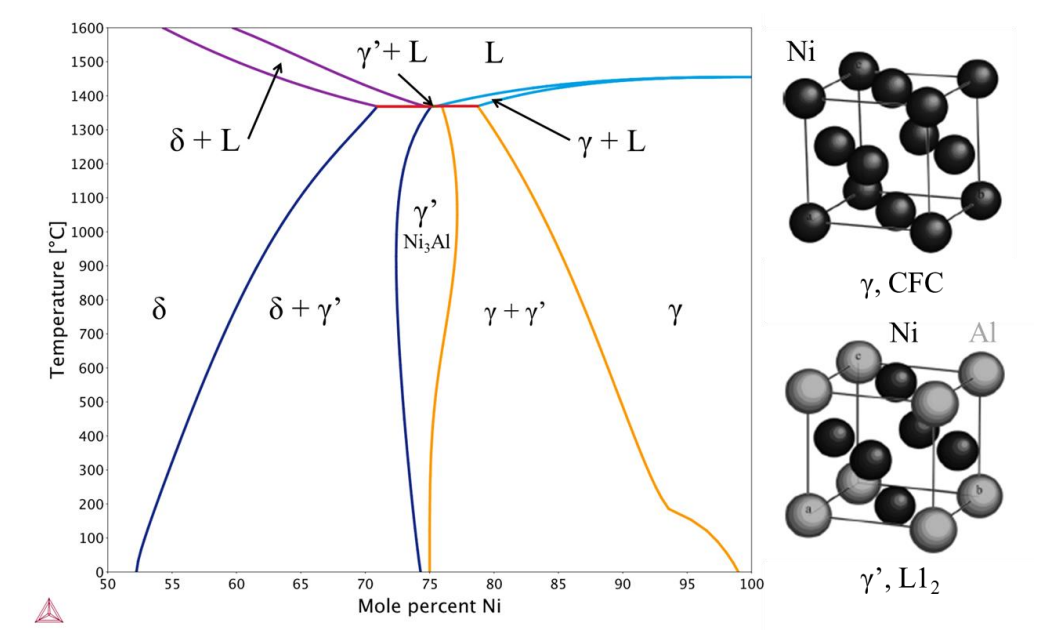
\includegraphics[width=0.75\textwidth]{images/diagramme_phase.png}
    \caption{Diagramme Ni-Al avec les structures cristallines des phases $\gamma$ et $\gamma'$}
    \label{fig:diagramme_phases_Ni_Al}
\end{figure}

% Quand on regarde le diagramme de phases nickel-aluminium, nous voyons que 
% lors de la solidification, le liquide va s'appauvrir en nickel et sa composition
% va tendre vers celle du liquide eutectique. Cela conduit donc à la formation de zones
% donc la composition est celle de l'assemblage $\gamma$/$\gamma'$, et d'autres zones 
% contenant uniquement la phase $\gamma'$ qui correspondent aux agrégats eutectiques.


Quant aux pores, leur apparition est liée à un flux trop faible de soluté 
dans les espaces inter-dendritiques, c'est-à-dire que la solidification de 
certaines zones se fait sans que le liquide ou la diffusion aient eu le 
temps de combler certains vides créés par la contraction du liquide qui
se refroidit. Nous avons donc un certain nombre de lacunes et de pores qui
apparaît ; ce nombre varie en fonction de la vitesse de refroidissement 
de la pièce.\\


Observons maintenant l'état des dendrites dans notre échantillon, grâce au 
traitement chimique à l'eau régale que nous avons effectué.\\ 


\begin{figure}[H]
    \centering
    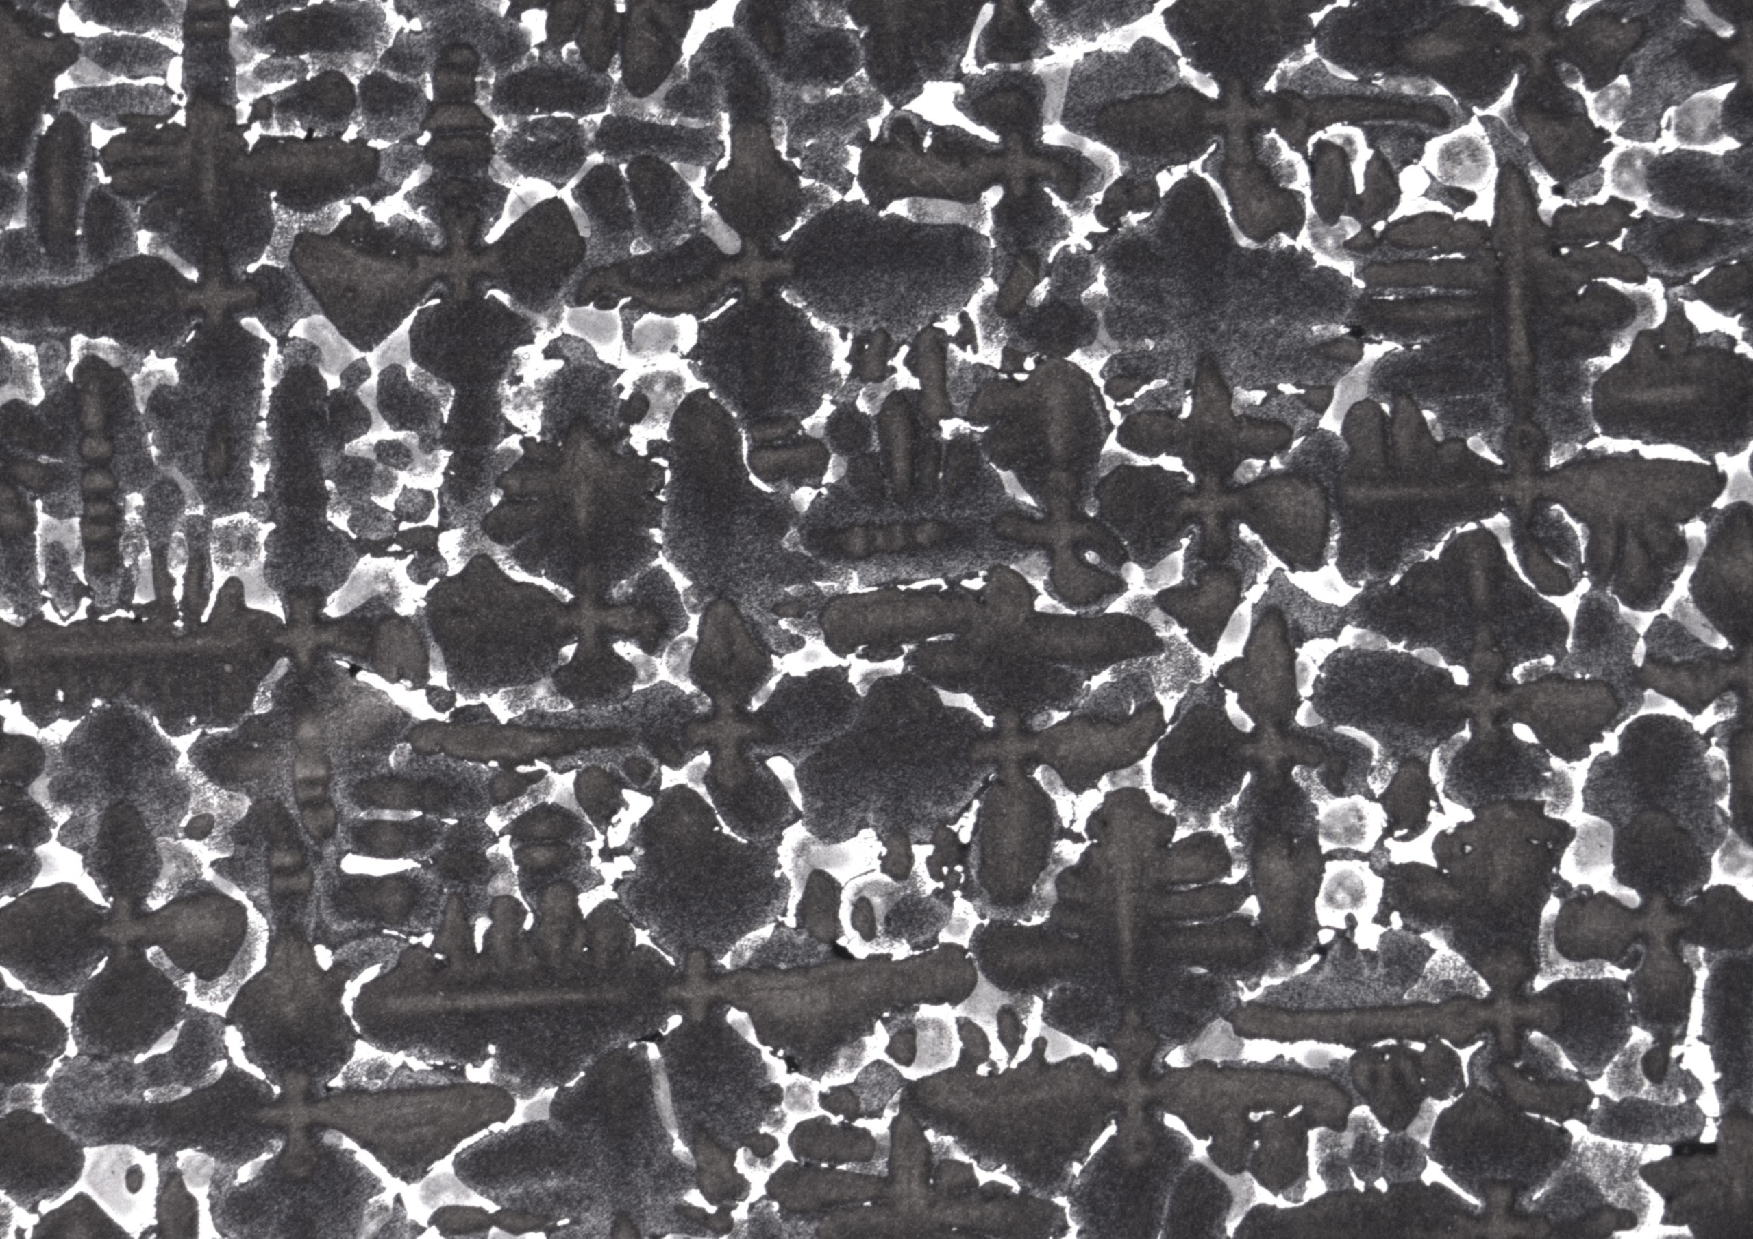
\includegraphics[width = 0.55\textwidth]{brut_dendrites.pdf}
    \caption{Observation des dendrites sur l'échantillon brut de fonderie
     au microsope optique, après traitement chimique à l'eau régale}
    \label{fig:brut_dendrites_optique}
\end{figure}

Nous obtenons un résultat clair : les dendrites (sombres, composées majoritairement
de phase $\gamma$) sont extrèmement développées et marquées en constrate de 
l'espace inter-dendritique (de couleur claire), qui a été attaqué par l'acide. 
Leur forme est dû au mécanisme de solidification successive de la pièce, 
lorsque le liquide se refroidit. Les dendrites croissent alors en partant 
de la base, et adoptent cette forme en sapin de Noël. Le matériau est donc inhomogène, 
ce qui nuit à ses qualités mécaniques. \\


Enfin, nous pouvons étudier nos clichés obtenus au microscope électronique à balayage
de la surface de l'échantillon brut de fonderie. 

\begin{figure}[H]
    \centering
    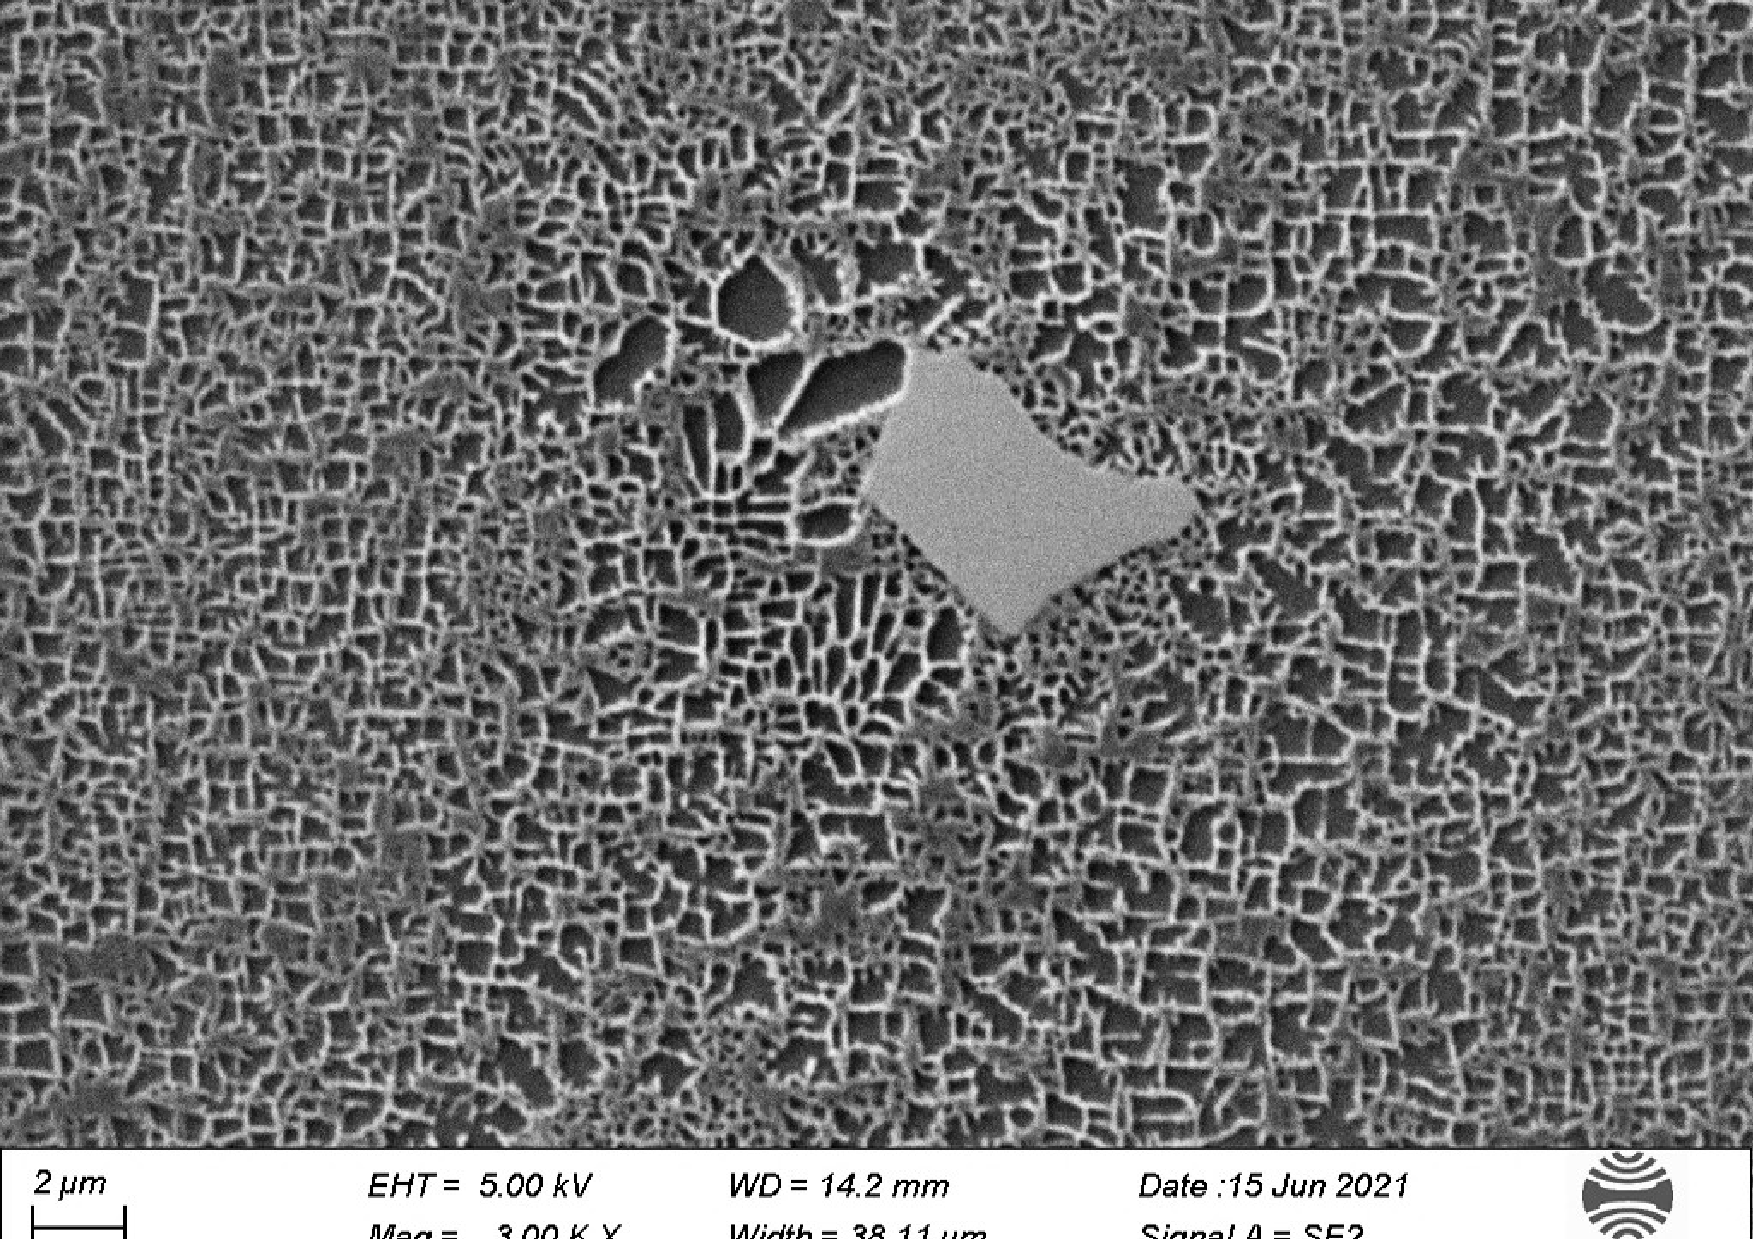
\includegraphics[width = 0.5\textwidth]{brut1912.pdf}
    \caption{Echantillon brut de fonderie vu au microscope électronique à balayage\\}
    \label{fig:brut_MEB}
\end{figure}

La microstructure de l'échantillon brut est désordonnée (bien que constituée d'un seul grain) :
nous avons en effet des polyèdres de phase $\gamma'$ liés par de la phase $\gamma$,
mais la microstructure est peu régulière. Nous voyons également un agrégat eutectique 
au centre de la figure \ref{fig:brut_MEB}.


\subsection*{Echantillon remis en solution}

Regardons maintenant notre échantillon après la remise en solution. 
Ce traitement consiste à réchauffer la pièce à très haute température (\SI{1300}{\celsius}),
mais en-dessous du point de fusion de l'alliage : aucun liquide n'est donc formé. 

Ce traitement a pour but d'homogénéiser la composition de l'alliage. En effet, nous avons 
vu différentes zones se solidifient à différents moments, ce qui place une partie de l'alliage
hors équilibre (comme par exemple les agrégats eutectiques). Le chauffage intense va également 
permettre d'accèlérer la diffusion dans l'alliage, et donc faciliter le mouvement des atomes 
(notamment les plus lourds comme le rhénium). 

Observons donc notre échantillon ayant subit une étape de remise en solution au microscope optique.

\begin{figure}[H]
    \centering
    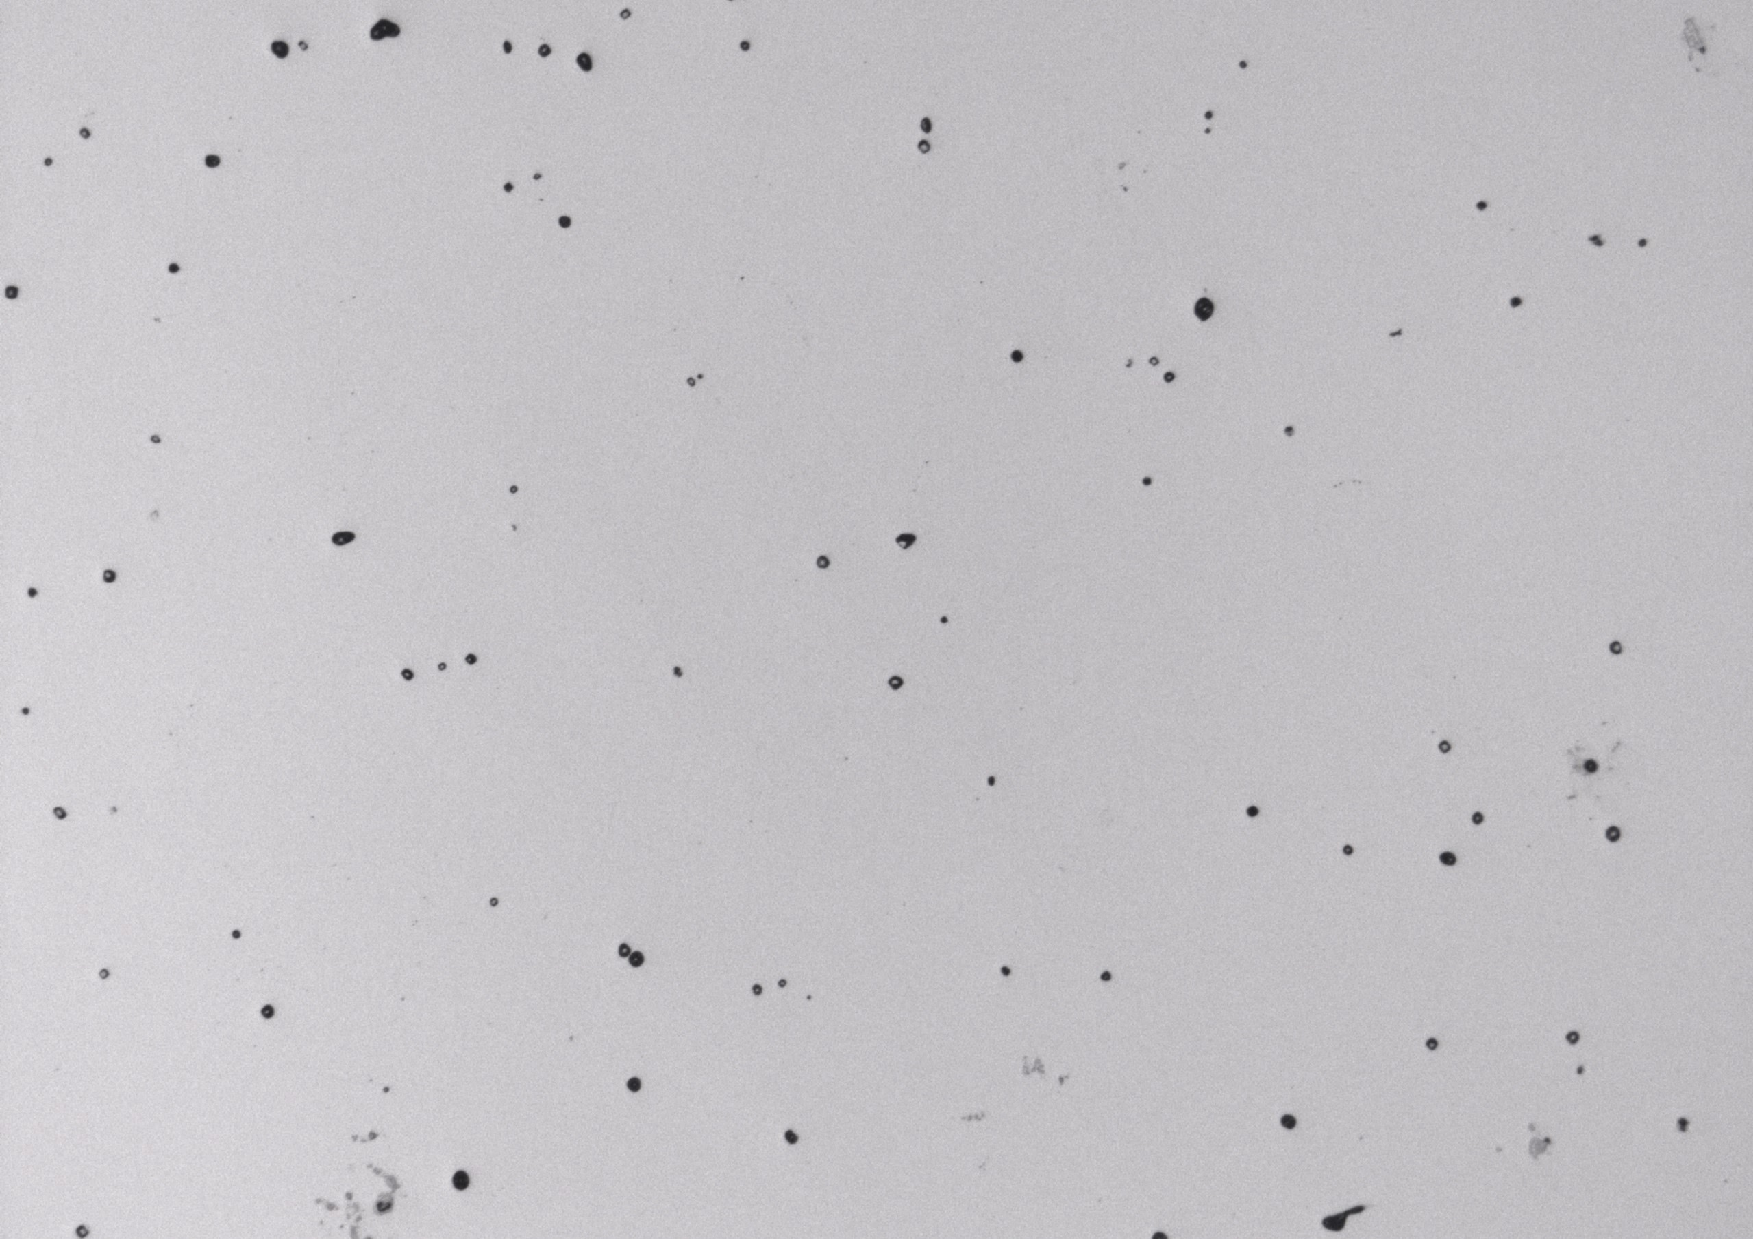
\includegraphics[width=0.55\textwidth]{images_optique/res.pdf}
    \caption{Echantillon après traitement de remise en solution}
    \label{fig:RES_optique}
\end{figure}

Nous voyons que les agrégats eutectiques, très visibles sur le brut, ont quasiment disparu.
Ils étaient en effet nettement hors équilibre et donc peu stables thermodynamiquement. 

Néanmoins, nous avons augmenté le nombre de pores. Cela est lié au fait que, la température 
augmentant, nous avons également augmenté la mobilité de tous les atomes et donc la possibilité
de former des pores en se refroidissant.\\

Il s'agit d'un effet indésirable du processus de remise en solution, d'autant plus que 
les deux traitements de revenu successifs ne parvienne pas à supprimer ces pores. 
Cependant, ce n'est pas un problème important car les bénéfices apportés par la diminution des 
agrégats eutectiques sont supérieurs, notamment en termes de résistance au fluage. \\

Nous obtenons les résultats suivants à l'aide d'ImageJ :

\begin{table}[H]
    \centering
    \caption{Proportion des différents défauts dans l'échantillon après remise en solution}
    \begin{tabular}{|c|c|}
        \hline
        \textbf{Type de défaut}  & \textbf{Proportion observée}  \\
        \hline
        Pore               & 0,525  \% \\
        Agrégat eutectique & 0,0041 \% \\
        \hline
    \end{tabular}
    \label{fig:proportion_defauts_RES}
\end{table}

Ces mesures corroborent nos observations visuelles.\\

Nous pouvons donc produire le graphique de comparaison suivant :


\begin{figure}[H]
    \centering
    % This file was created by tikzplotlib v0.9.8.
\begin{tikzpicture}

\definecolor{color0}{rgb}{0.12156862745098,0.466666666666667,0.705882352941177}
\definecolor{color1}{rgb}{1,0.498039215686275,0.0549019607843137}

\begin{axis}[
legend cell align={left},
legend style={
  fill opacity=0.8,
  draw opacity=1,
  text opacity=1,
  at={(0.03,0.97)},
  anchor=north west,
  draw=white!80!black
},
tick align=outside,
tick pos=left,
title={Évolution des défauts dans les échantillons\\selon les traitements thermiques appliqués},
x grid style={white!69.0196078431373!black},
xlabel={Etape de traitement thermique de l'échantillon},
title style = {align=center},
xmin=-0.23, xmax=1.53,
xtick style={color=black},
xtick={0.15,1.15},
xticklabels={Brut,Remis en solution},
y grid style={white!69.0196078431373!black},
ylabel={Proportion surfacique\\du type de défaut},
% ylabel style={text width=4cm},
ylabel style={align=center},
ymin=0, ymax=0.55125,
ytick style={color=black},
ytick={0,0.1,0.2,0.3,0.4,0.5,0.6},
yticklabels={0.00\%,0.10\%,0.20\%,0.30\%,0.40\%,0.50\%,0.60\%}
]
\draw[draw=none,fill=color0,fill opacity=0.9] (axis cs:-0.15,0) rectangle (axis cs:0.15,0.34);
\addlegendimage{ybar,ybar legend,draw=none,fill=color0,fill opacity=0.9};
\addlegendentry{Pores}

\draw[draw=none,fill=color0,fill opacity=0.9] (axis cs:0.85,0) rectangle (axis cs:1.15,0.525);
\draw[draw=none,fill=color1,fill opacity=0.9] (axis cs:0.15,0) rectangle (axis cs:0.45,0.252);
\addlegendimage{ybar,ybar legend,draw=none,fill=color1,fill opacity=0.9};
\addlegendentry{Agrégats eutectiques}

\draw[draw=none,fill=color1,fill opacity=0.9] (axis cs:1.15,0) rectangle (axis cs:1.45,0.0041);
\end{axis}

\end{tikzpicture}

    \caption{Évolution de la proportion surfacique des défauts dans les 
    échantillons selon les traitements thermiques appliqués\\}
    \label{fig:evolution_proportion_defauts_brut_RES}
\end{figure}

À nouveau, nous pouvons étudier notre échantillon après l'attaque chimique, 
afin de déterminer l'influence de la remise en solution sur les dendrites.\\

\begin{figure}[H]
    \centering
    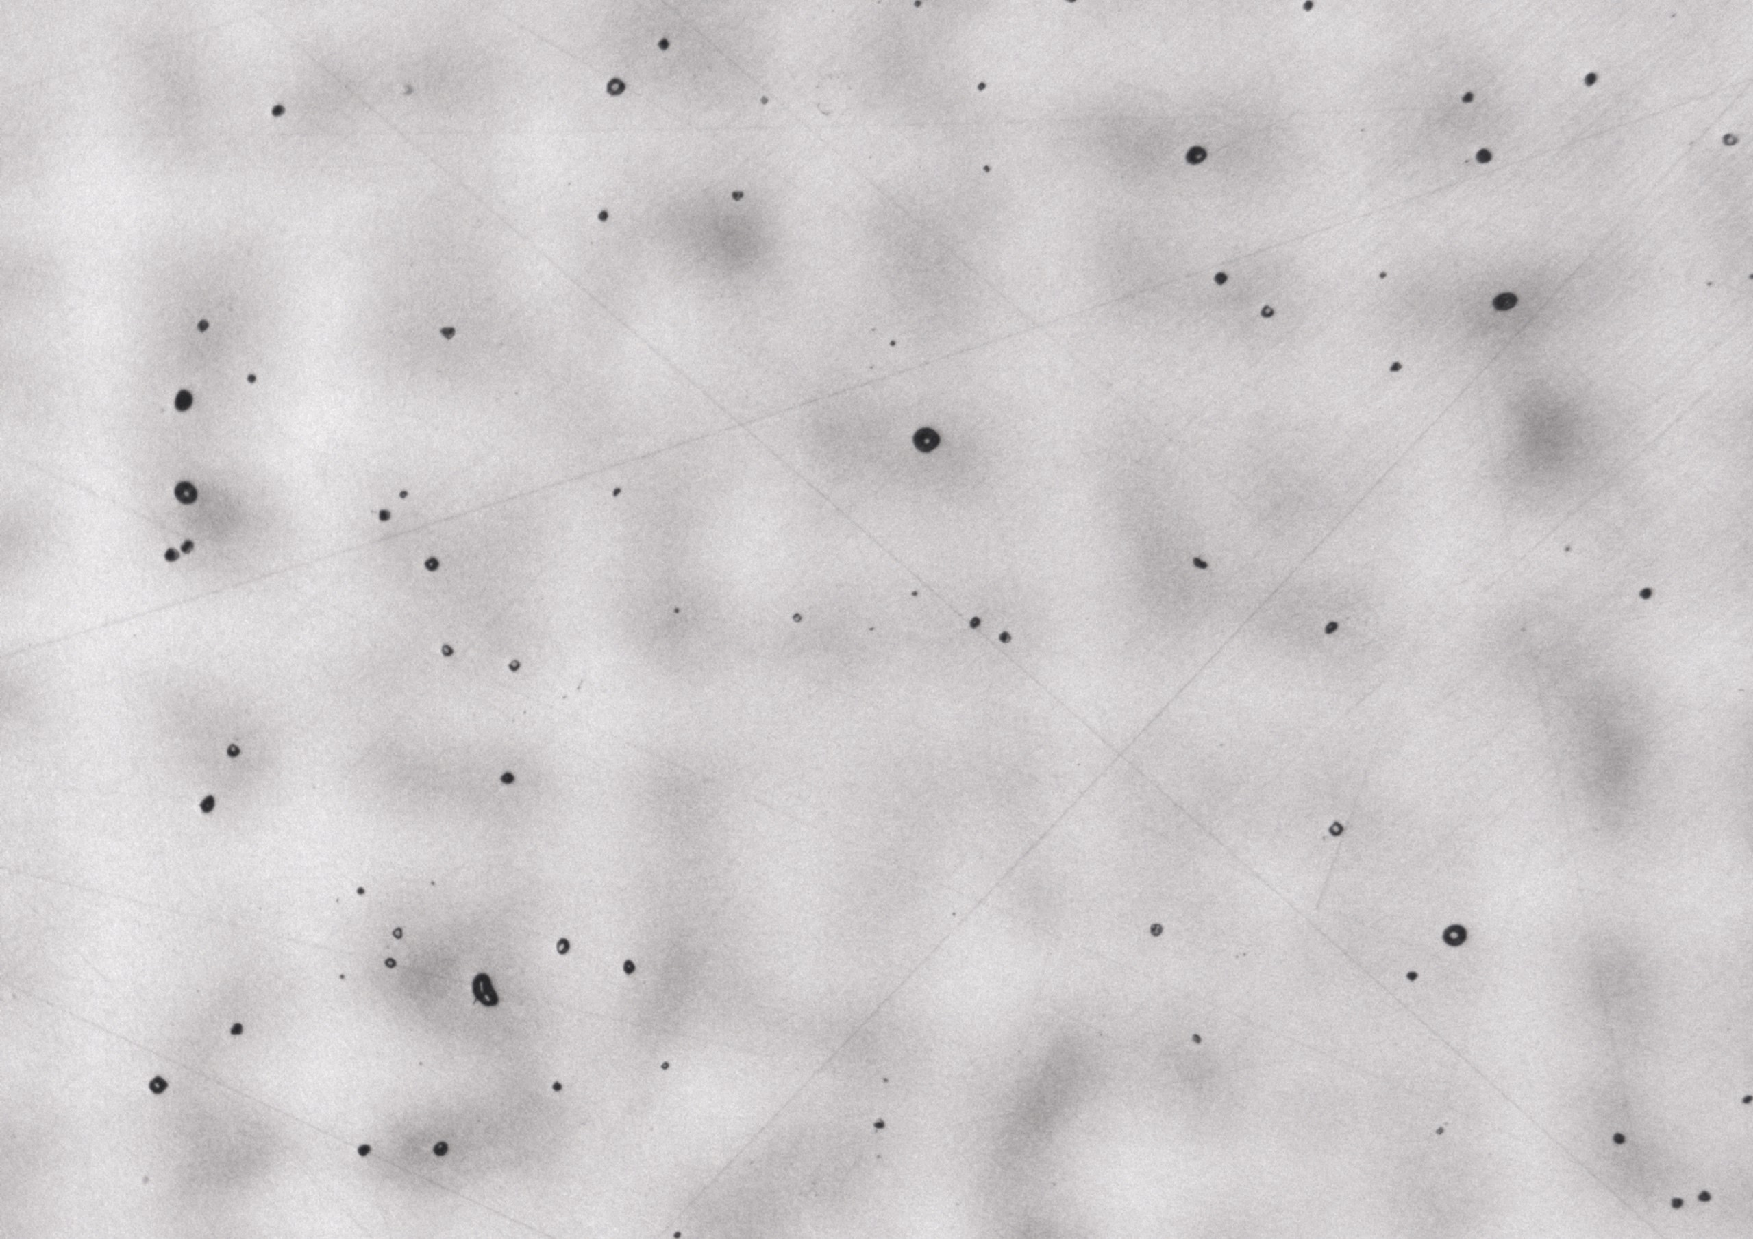
\includegraphics[width = 0.55\textwidth]{images_optique/res_dendrites.pdf}
    \caption{Observation des dendrites sur l'échantillon ayant subi une remise en solution
    au microsope optique, après traitement chimique à l'eau régale\\}
    \label{fig:RES_dendrites_optique}
\end{figure}

Nous observons que, bien que la forme originelle des dendrites soit encore discernable, 
celle-ci est beaucoup plus atténuée. Nous avons donc réussi à homogénéiser nettement
la composition chimique de notre pièce, en enlevant d'une part les agrégats eutectiques, 
et d'autres part en "adoucissant" la frontière entre dendrites et espaces inter-dendritiques.\\

Enfin, étudions les images obtenues au microscope électronique à balayage.

\begin{figure}[H]
    \centering
    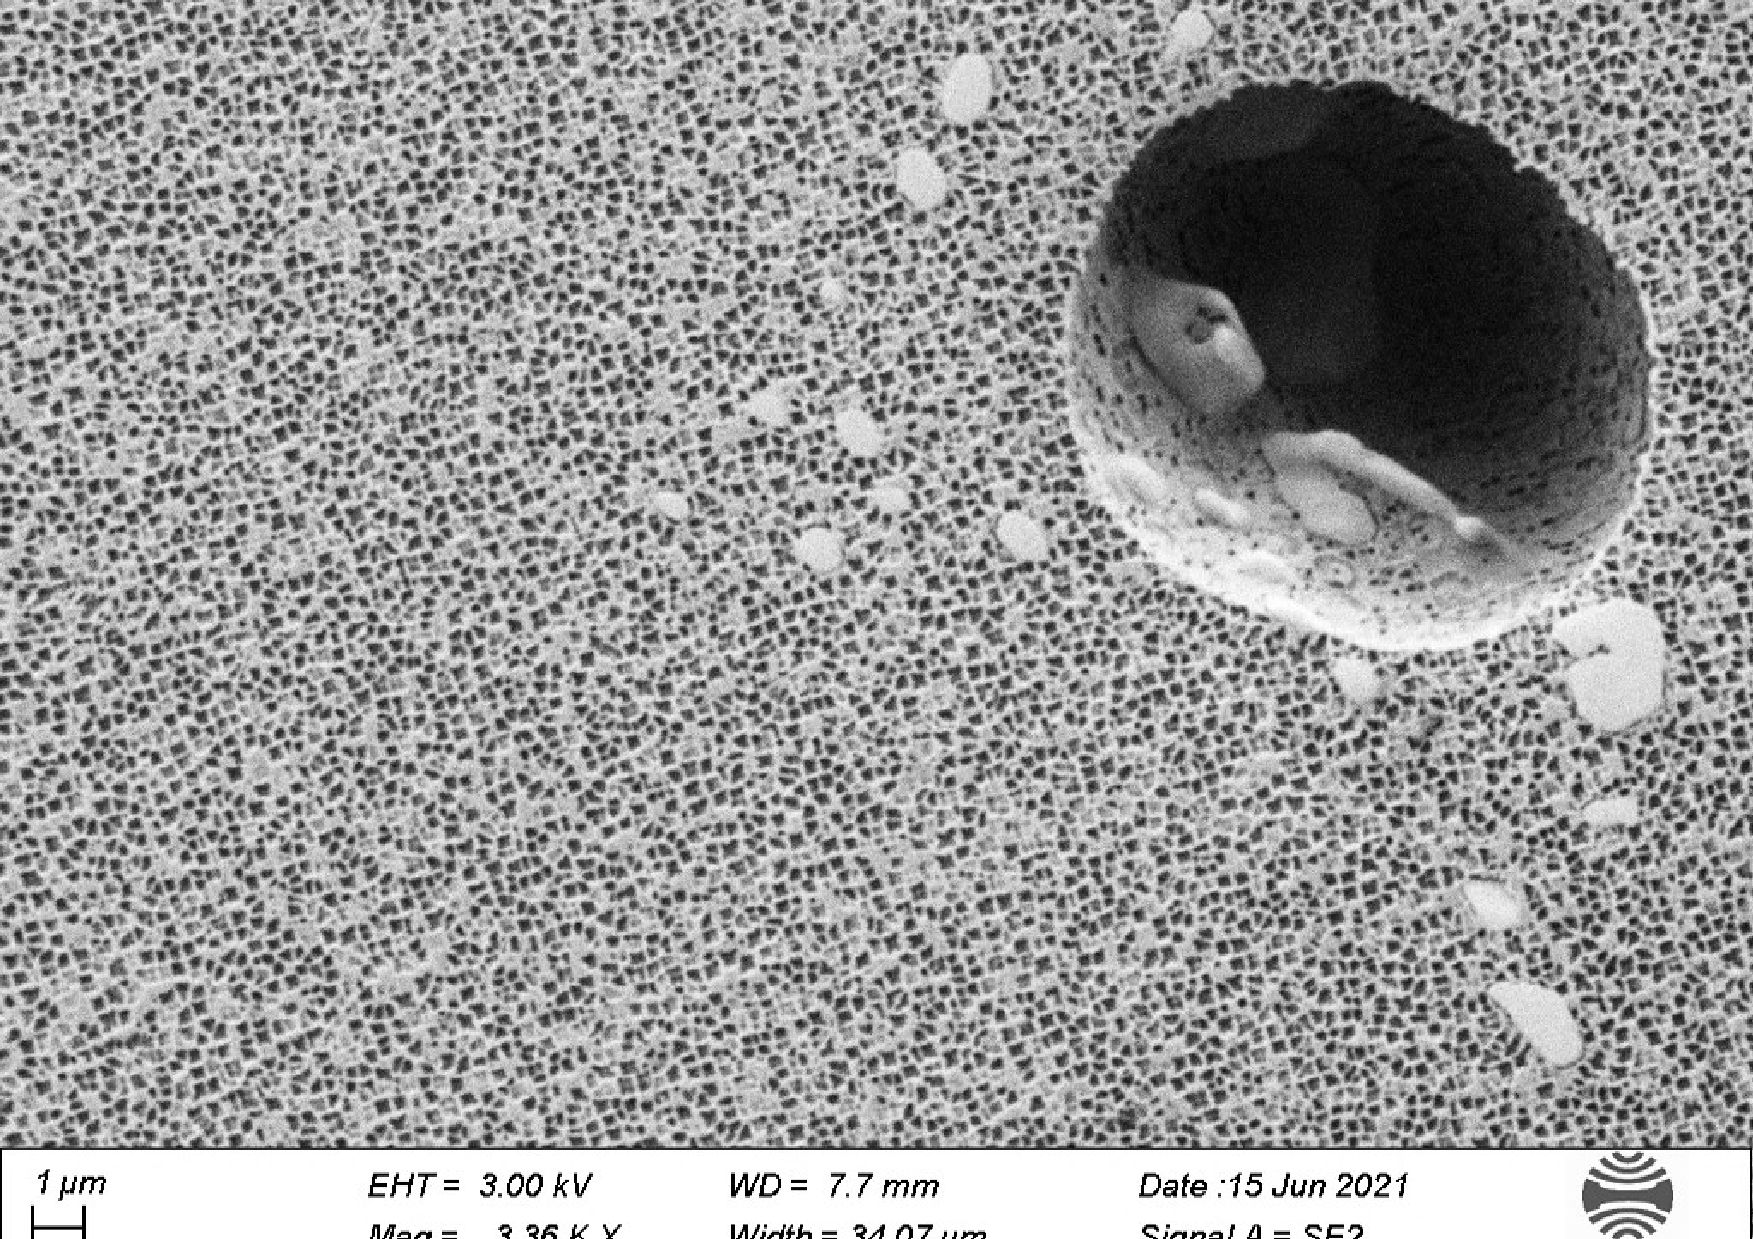
\includegraphics[width=0.6\textwidth]{images_meb/RS1913.pdf}
    \caption{Echantillon observé au microsope électronique à balayage, 
    après traitement de remise en solution\\}
    \label{fig:RES_MEB}
\end{figure}

Nous voyons sur ce cliché que, malgré la présence d'un pore, la microstructure
est beaucoup plus régulière, avec des cuboïdes de phase $\gamma'$, dure, reliés
par des "bandes" de phase $\gamma$, beaucoup plus ductile. C'est la combinaison 
de ces deux phases qui apporte ses propriétés à l'alliage : résistance au fluage
(un seul grain, peu de lacunes), résistance mécanique (à la fois résistant et souple).\\

En comparaison, voici les clichés de la structure finale, après tous les 
traitements thermiques :\\

\begin{figure}[htbp]
    \centering
    \begin{minipage}{0.45\textwidth}
        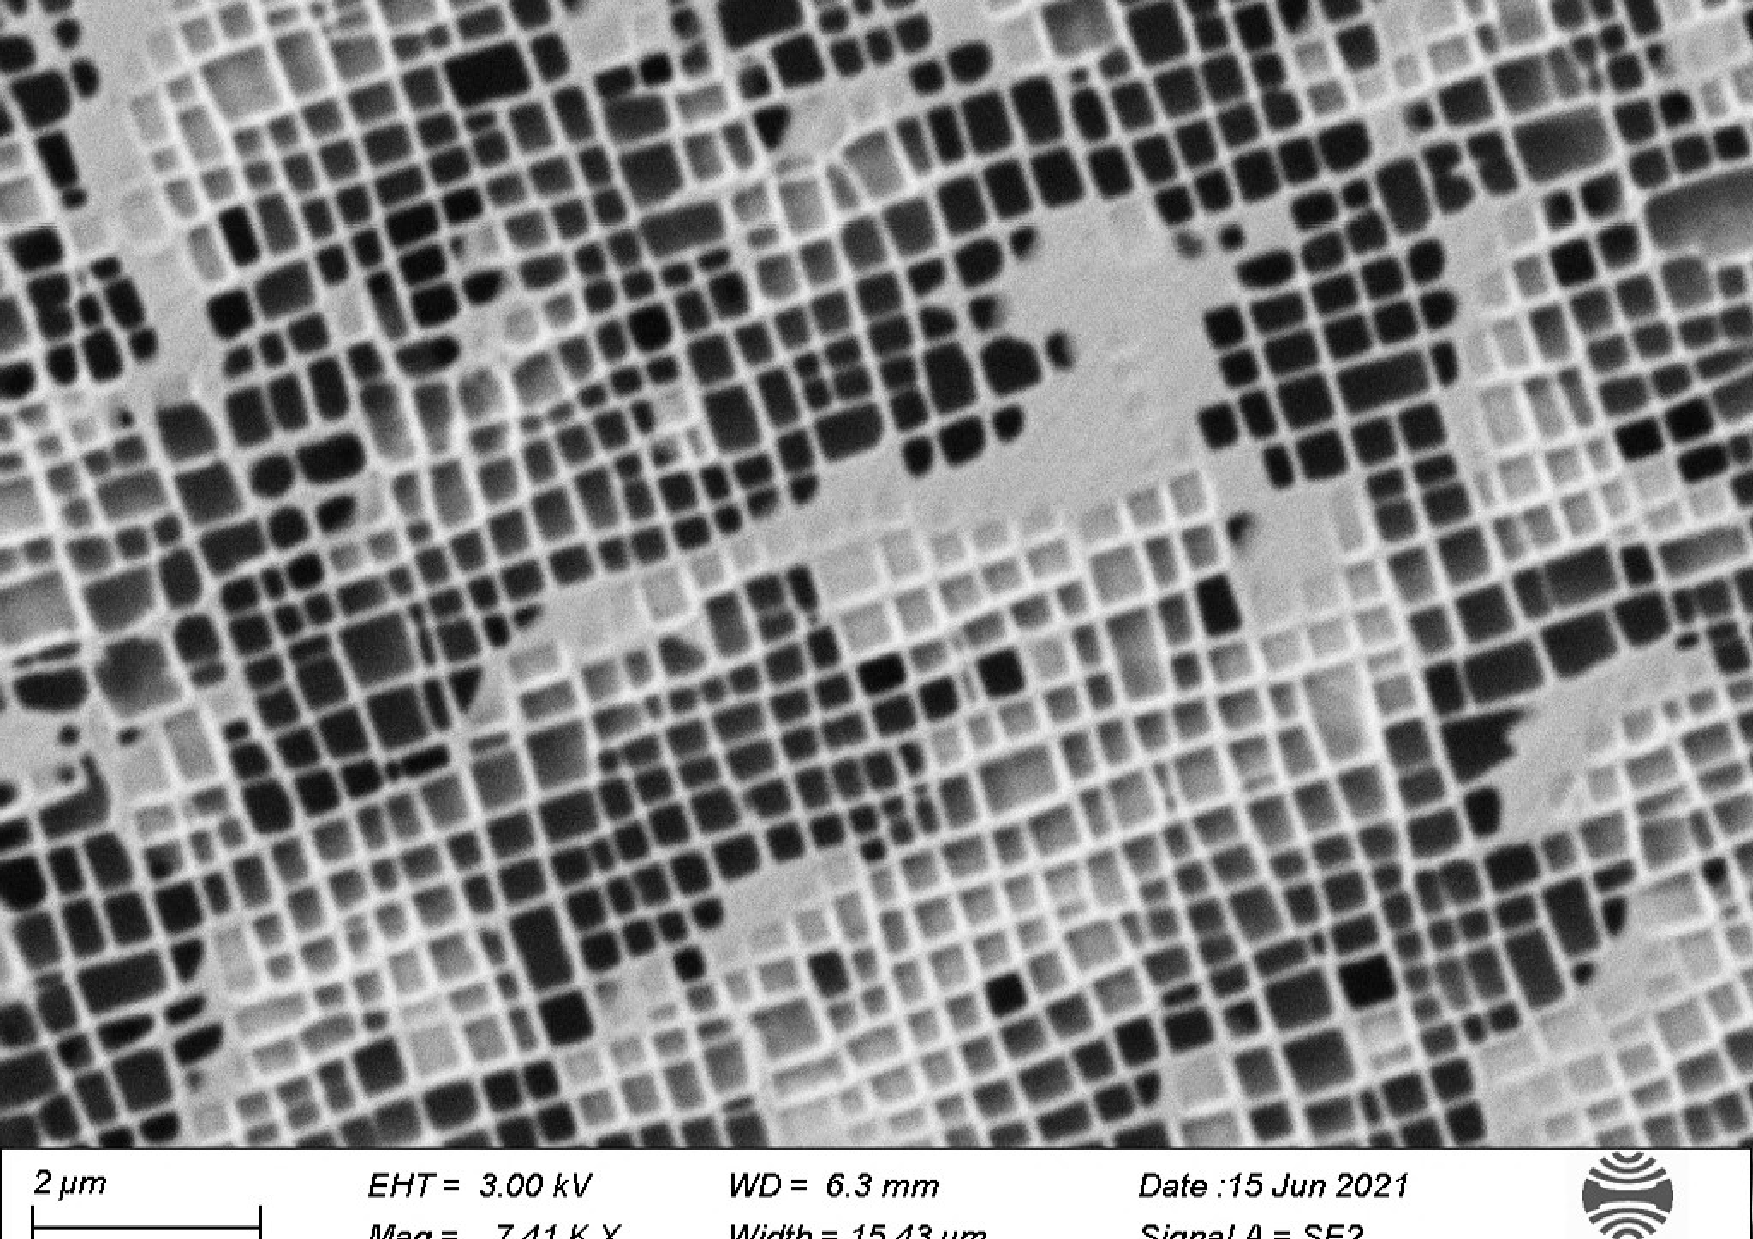
\includegraphics[width=0.9\textwidth]{images_meb/TTH1914.pdf}
    \end{minipage}%
    \begin{minipage}{0.45\textwidth}
        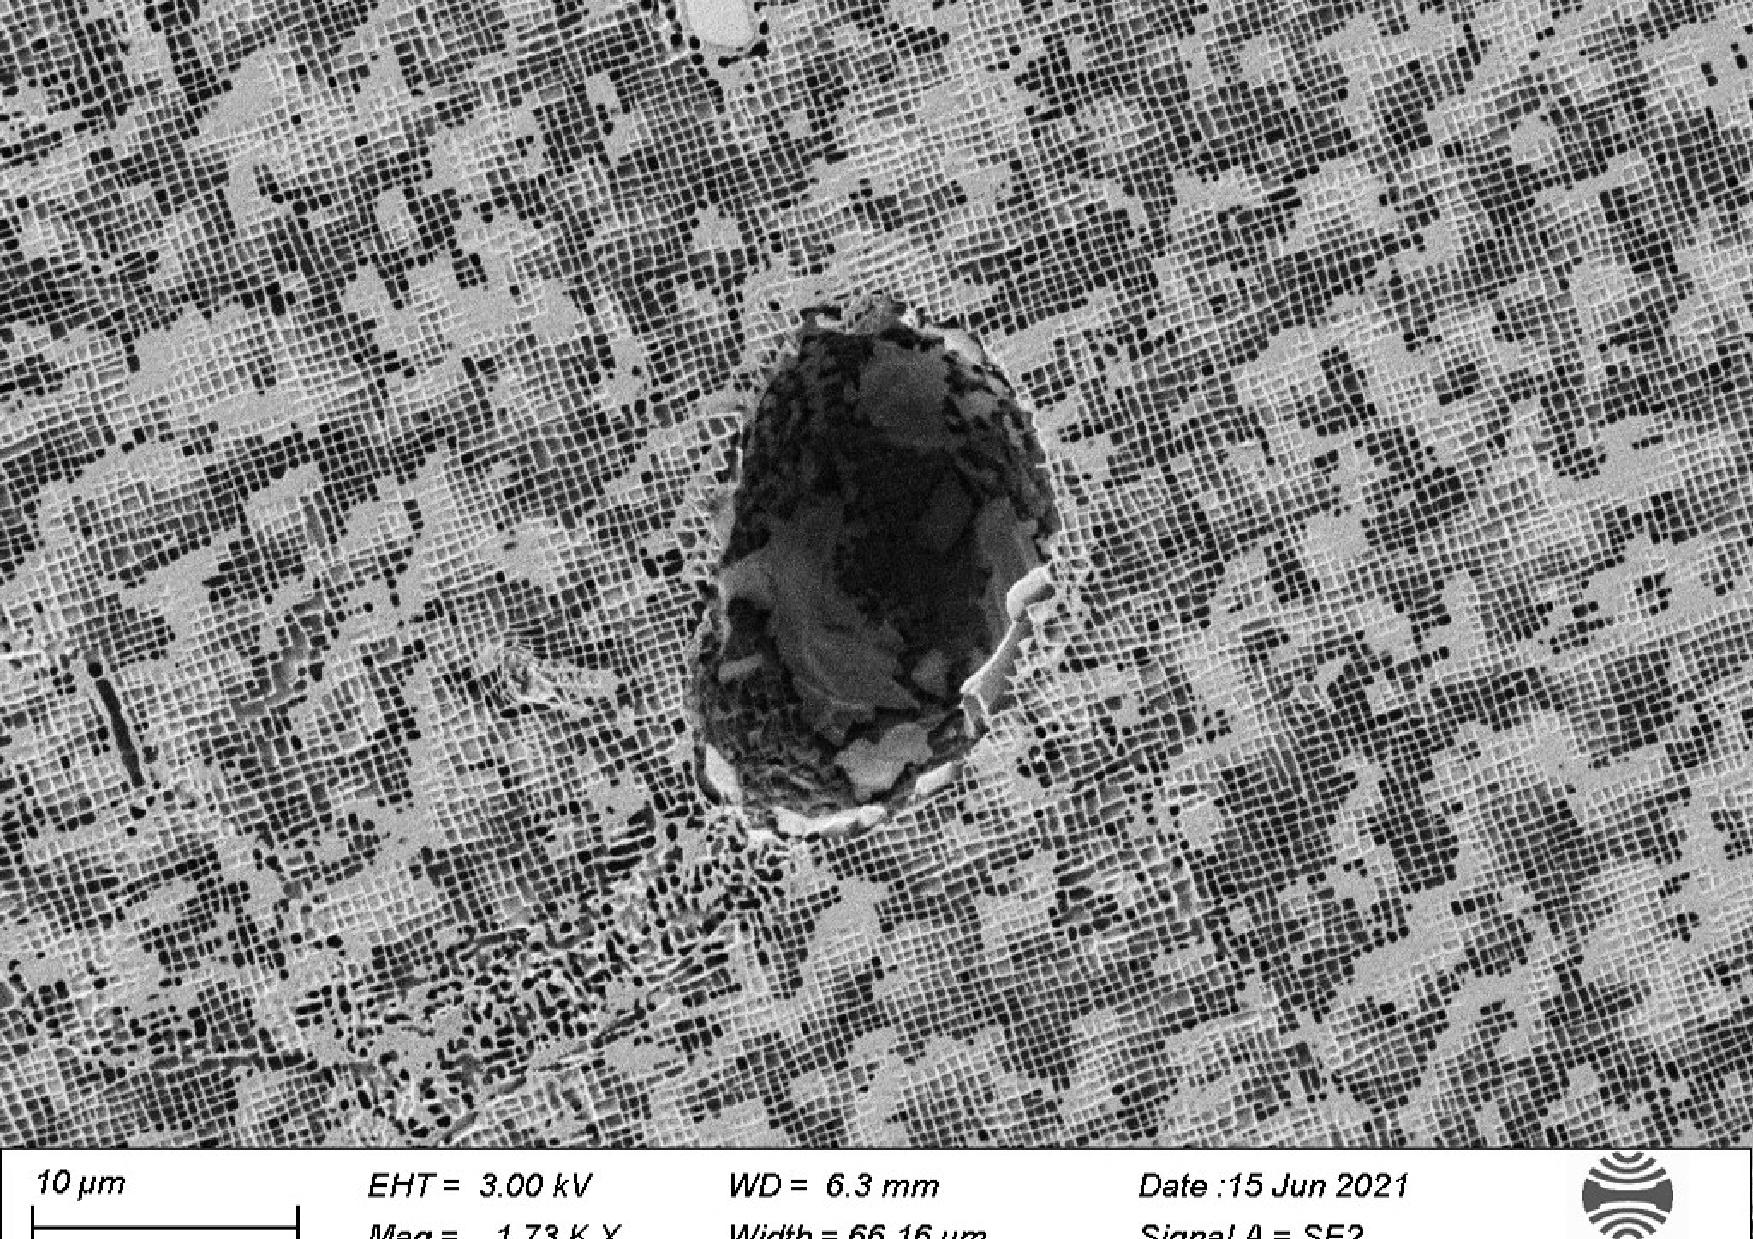
\includegraphics[width=0.9\textwidth]{images_meb/TTH1915.pdf}
    \end{minipage}%    
    \caption{Echantillon ayant subi un traitement thermique complet, 
    vu au microscope électronique à balayage}
    \label{fig:complet_MEB}
\end{figure}

La structure finale est extrèmement régulière.\\

\subsection*{Conclusion sur les traitements thermiques}

La remise en solution permet donc d'améliorer nettement la qualité du matériau en
homogénéisant sa structure et en diminuant drastiquement le nombre d'agrégats
eutectiques, qui sont des endroits autours desquels la concentration n'est pas 
homogène, et dont la composition ne correspond pas au mélange $\gamma$/$\gamma'$
que l'on veut obtenir pour garantir les bonnes propriétés mécaniques de la pièce 
(résistance au fluage, résistance aux dislocations et déformations).





\section*{Conclusion scientifique}
Les différentes observations au microscope optique et au MEB ont révélé le comportement des différentes phases, des dendrites et des pores face aux différents traitements thermiques. 
\\
\\
Nous avons pu constater au MEB que les micro-structures sont effectivement différentes suivant les différents traitements appliqués. Nous avons en particulier estimé les tailles de précipités ainsi que leur fraction surfacique. En comparaison avec l’état initial (brut), les précipités après traitements thermique semblent plus organisés et alignés sur les clichés MEB. Il apparaît également une diminution de la part d'agrégats eutectiques et ce dès le premier traitement thermique.
\\
\\
Un des défauts résultant du procédé de fonderie, et qui a déjà été évoqué, est la présence d’une hétérogénéité chimique due à la croissance dendritique qui persiste malgré l’application de traitements thermiques. Les atomes plus lourd (Ta, W, Re) qui diffusent plus lentement n’ont pas le temps durant la remise en solution de se répartir de manière homogène. Des analyses EPMA sur un super-alliage après traitement thermique montrent la disparité de composition qu’il est possible de retrouver dans les zones dendritiques et interdendritiques.
Cette ségrégation résiduelle induit une précipitation légèrement différente dans chacune des zones, qui va modifier le désaccord paramétrique naturel, qui dépend de la composition de chacune des phases. Ceci influence le comportement du matériau, notamment en fluage où une densité de dislocations plus importante a été observée dans le cœur des dendrites.
Durant la solidification, le flux de soluté n’est parfois pas assez suffisant dans les zones interdendritiques laissent place à des vides appelées pores ou retassures. En général, ils sont de forme arrondie et distants de l'ordre de l'espace interdendritique secondaire (150 à 550 $\mu$m) avec une dimension maximale comprise entre 40 $\mu$m et 60 $\mu$m pour un rayon moyen de 5$\mu$m . Lorsque les zones interdendritiques sont contigües ou interconnectées, des cavités plus grandes peuvent être observées. Pendant une sollicitation thermomécanique, un champ de concentration de contraintes est alors présent autour des pores, pouvant aller jusqu’à l’amorçage d’une fissure.

\section*{Conclusion générale}
Nous avons trouvé très enrichissante l'opportunité de rencontrer des doctorants au cours de cette journée.
Leur manière d'expliquer et d'appréhender la mécanique des matériaux est bien différente de celle des 
enseignants et nous avons tous senti que cette double approche a été très bénéfique pour notre apprentissage 
de la matière. Nous sommes aussi conscients de la chance que nous avons eu de passer une journée entière avec 
des chercheurs qui étaient heureux de répondre à toutes nos questions et de nous partager leur domaine de 
recherche en nous accompagnant tant sur la partie théorique qu'expérimentale. 

Cette journée a été très intense intellectuellement et cela a été très satisfaisant de pouvoir, à la fin de 
la journée, appréhender un sujet complexe sur lequel on ne connaissait encore rien le matin. Nous saluons 
pour cela la très grande pédagogie de nos encadrants qui ont su nous faire digérer les concepts de manière 
progressive tout en nous faisant percevoir une logique globale que nous ne quittions jamais. L'approche 
expérimentale du problème que nous avons pu mener était également précieuse pour notre compréhension puisque 
voir les choses de ses propres yeux aide beaucoup à l'apprentissage.

Enfin, c'était pour nous trois notre première expérience dans un laboratoire de recherche. Nous avons été 
impressionnés par les équipements que nous avons été amenés à utiliser, notamment le MEB. Pour ma part 
j'avais fait mon TPE sur la cristallographie et la diffraction aux rayons X et je n'avais pu voir un tel 
dispositif à l'époque.

En bref cette journée était bien supérieure à une journée de cours, tant au niveau de l'enrichissement 
personnel que de l'apprentissage scientifique.






\end{document}